\documentclass{WCCM-ECCOMAS_2026_Full_Paper}

\usepackage{graphicx}
\usepackage{amsmath}
\usepackage{amssymb}
\usepackage{booktabs}
\usepackage{xcolor}
\usepackage{float}
\usepackage{tikz}
\usetikzlibrary{arrows.meta,positioning,fit,calc}
\usepackage[colorlinks=true,linkcolor=blue,urlcolor=blue,citecolor=blue]{hyperref}

% ---------------------------------------------------------------
% Title — all caps per ECCOMAS format
% ---------------------------------------------------------------
\title{Symbolic Shock Sensor for Physics-Informed Mixture-of-Experts Surrogates in Transonic Aerodynamics}

\author{Marta Arnabat-Martín$^{*}$, Andrés Mateo-Gabín$^{\P}$, Sven A. Lanzan-Ferran$^{\P}$ and Gonzalo Rubio$^{\dag}$}
\shortauthors{Marta Arnabat-Martín}

\address{%
$^{*}$ Flight Physics Technology and Capability\\
Airbus Defence and Space, C/ Aviocar 2, 28906 Getafe, Madrid, Spain \\
Universidad Politécnica de Madrid, Plaza Cardenal Cisneros, 3, Madrid, 28040, Spain\\
e-mail: marta.arnabt-martin@airbus.com \\[12pt]

$^{\P}$ Flight Physics Technology and Capability\\
Airbus Defence and Space, C/ Aviocar 2, 28906 Getafe, Madrid, Spain \\
e-mail: andres.mateo@airbus.com \\
e-mail: sven\_agustin-lanzan@airbus.com \\[12pt]
$^{\dag}$ Applied Mathematics department - School of aeronautics\\
Universidad Politécnica de Madrid, Plaza Cardenal Cisneros, 3, Madrid, 28040, Spain\\
Center of Computational Simulation, Universidad Politécnica de Madrid, Campus de Montegancedo, Boadilla del Monte, 28660 Madrid, Spain

}

\keywords{shock capture, mixture of experts, Gumbel-Softmax routing,
symbolic regression, physics-informed machine learning, RANS surrogate}

\summary{A physics-aware machine learning surrogate is presented for the
prediction of aerodynamic surface coefficients $[C_p, C_{fx}, C_{fy},
C_{fz}]$ on a transonic transport configuration, requiring no CFD solver
at inference.  The model, AeroSurrogate, couples a lightweight shock
indicator network with a shock-gated Mixture of Experts: four smooth
experts capture regime-dependent aerodynamic loading, while a dedicated
shock expert contributes an additive residual scaled by the predicted
shock probability, providing an explicit mechanism for the pressure
discontinuity that smooth networks systematically blur.  Expert routing
uses a Mach-gated Gumbel-Softmax that applies stochastic exploration
only in the transonic regime.  All shock labels are derived from real
RANS surface pressures via the critical pressure coefficient---no
isentropic pseudo-labels are used.  Post-training, the learned shock
criterion is distilled by symbolic regression into the closed-form
expression $\tanh(\exp(C_p^{\mathrm{crit}}/\eta))$, where $\eta$ is the
normalised span position; retraining with this frozen symbolic gate
yields aerodynamic accuracy identical to the neural gate.  Trained on
RANS surface data of the ONERA CRM WBPN database spanning Mach
$0.30$--$0.96$ and angle of attack up to $\pm 15^{\circ}$, the model achieves
$R^{2}=0.951$ for $C_p$ and $R^{2}\approx 0.85$ for the skin-friction
components over more than four million held-out test points, with only
$3\times 10^{5}$ parameters.}

\begin{document}
\maketitle

% ================================================================
\section{INTRODUCTION}
% ================================================================

Transonic aerodynamic flows are characterised by the coexistence of
subsonic and supersonic regions separated by shock waves.  In cruise
configurations, normal shocks on wing surfaces produce strong adverse
pressure gradients that drive boundary-layer thickening, flow
separation, and buffet onset---phenomena central to the determination
of drag-divergence Mach number and the structural loads
envelope~\cite{Vassberg2008,Levy2013}.  Fast and accurate prediction
of surface aerodynamic loading across the full flight envelope is
therefore a fundamental requirement for aerodynamic analysis pipelines
that must operate at high frequency, such as adjoint-based shape
optimisation, digital-twin monitoring, or real-time loads estimation.

Reynolds-Averaged Navier--Stokes (RANS) solvers provide physical
ground truth for shock structure but at a computational cost of
$\mathcal{O}(10^{3}$--$10^{4})$ CPU-hours per operating condition.
Machine learning (ML) surrogate models have emerged as a practical
alternative for rapid aerodynamic
prediction~\cite{Han2018,Bhatnagar2019,Sekar2019}.  A central
challenge in transonic aerodynamics is regime non-uniformity: the
relationship between surface geometry, flight condition, and
aerodynamic loading changes qualitatively across subsonic, transonic,
and separated flow regimes.  A single multi-layer perceptron (MLP)
trained on data spanning all regimes learns a smooth interpolant that
systematically blurs shock discontinuities, underestimating peak
suction and misrepresenting the pressure-recovery gradient aft of the
shock (Figure~\ref{fig:pathology}).  This smoothing pathology is
structural: a smooth network can
only approximate a step change in $C_p$ with an error proportional to
its activation range, and gradient-based training actively favours
the smeared solution because it reduces average error over the
predominantly smooth surface.

\begin{figure}[ht]
\centering
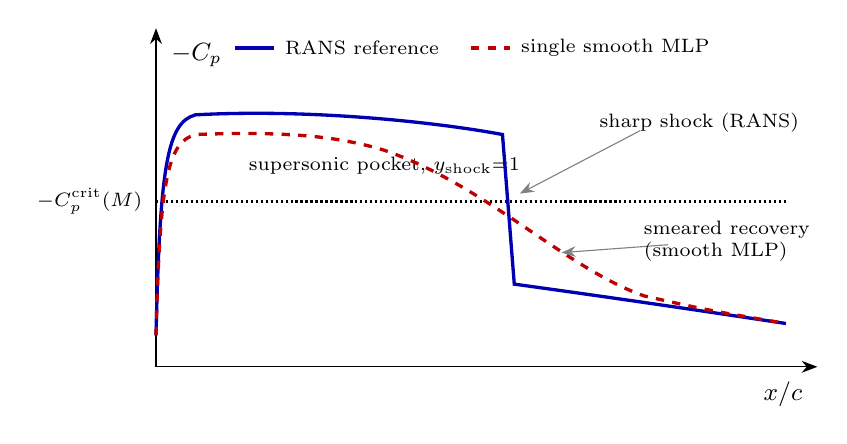
\begin{tikzpicture}[font=\small, x=1cm, y=1cm]
% Axes
\draw[-{Stealth[length=2mm]}] (0,0) -- (8.4,0) node[below left=1mm]{$x/c$};
\draw[-{Stealth[length=2mm]}] (0,0) -- (0,4.3) node[below right=1mm]{$-C_p$};
% Sonic threshold
\draw[densely dotted, thick] (0,2.1) -- (8,2.1);
\node[anchor=east] at (-0.05,2.1)
  {\scriptsize $-C_p^{\mathrm{crit}}(M)$};
\node[align=center] at (2.9,2.55)
  {\scriptsize supersonic pocket, $y_{\mathrm{shock}}{=}1$};
% RANS curve
\draw[very thick, blue!70!black]
  (0,0.4) .. controls (0.05,2.6) and (0.15,3.1) .. (0.5,3.2)
  .. controls (2.0,3.28) and (3.6,3.1) .. (4.4,2.95)
  -- (4.55,1.05)
  .. controls (6.0,0.85) and (7.0,0.7) .. (8,0.55);
% Smooth MLP curve
\draw[very thick, red!75!black, dashed]
  (0,0.4) .. controls (0.05,2.4) and (0.15,2.85) .. (0.5,2.95)
  .. controls (1.8,3.0) and (2.4,2.9) .. (2.9,2.75)
  .. controls (4.2,2.3) and (5.2,1.25) .. (6.2,0.9)
  .. controls (7.0,0.72) .. (8,0.55);
% Annotations
\draw[-{Stealth[length=1.8mm]}, gray] (6.15,3.0) -- (4.62,2.2);
\node[align=left] at (6.9,3.1) {\scriptsize sharp shock (RANS)};
\draw[-{Stealth[length=1.8mm]}, gray] (6.5,1.55) -- (5.15,1.45);
\node[align=left] at (7.25,1.6) {\scriptsize smeared recovery\\[-3pt]
  \scriptsize (smooth MLP)};
% Legend
\draw[very thick, blue!70!black] (1.0,4.05) -- (1.5,4.05)
  node[right, black]{\scriptsize RANS reference};
\draw[very thick, red!75!black, dashed] (4.0,4.05) -- (4.5,4.05)
  node[right, black]{\scriptsize single smooth MLP};
\end{tikzpicture}
\caption{Illustrative sketch of the shock-smoothing pathology:
  chord-wise $-C_p$ distribution on the upper wing in transonic flow.
  A single smooth MLP (dashed) blurs the sharp shock of the RANS
  reference (solid), underestimating peak suction and smearing the
  pressure recovery.  Points with $C_p < C_p^{\mathrm{crit}}$ (above
  the dotted line) form the supersonic pocket and define the shock
  label of Eq.~(\ref{eq:labels}).}
\label{fig:pathology}
\end{figure}

Existing ML shock indicators address discontinuity detection at the
volumetric field level.  Ray and Hesthaven~\cite{Ray2018,Ray2019}
pioneered neural network troubled-cell indicators for finite-element
solution fields; Discacciati et al.~\cite{Discacciati2020} and
Schwander et al.~\cite{Schwander2021} extended these with
convolutional architectures, and Morgan et al.~\cite{Morgan2020}
developed field-level indicators for Lagrangian hydrodynamics.  Two
limitations are shared across these approaches: (i)~they require
volumetric field data inaccessible in the surface-only measurement
context of experimental aerodynamics or flight test, and (ii)~they
commonly rely on pseudo-labels derived from isentropic assumptions
applied to input features, introducing a definitional circularity.
Physics-informed neural networks~\cite{Raissi2019,Karniadakis2021}
offer an alternative route but require embedding governing equations
explicitly and are computationally intensive to train.

The interpretability of ML models for physical discovery constitutes
a parallel active frontier.  Symbolic regression (SR)
methods---SINDy~\cite{Brunton2016}, Eureqa~\cite{Schmidt2009}, and
PySR~\cite{Cranmer2020}---have demonstrated that compact,
human-readable governing equations can be recovered from data, and
recent benchmarks~\cite{LaCava2021,Angelis2023} have shown their
maturity across physical domains.  However, their application to
aerodynamic shock physics at industrial scale, and in particular
their use \emph{inside} a deployed surrogate as a functional
component rather than a post-hoc explanation, has not been
demonstrated.

This work addresses both gaps simultaneously with
\emph{AeroSurrogate}, a compact ($3\times 10^{5}$-parameter)
architecture that predicts the four surface aerodynamic coefficients
$[C_p, C_{fx}, C_{fy}, C_{fz}]$ at every mesh node of a transonic
transport configuration from surface geometry and flight condition
alone.  The four main contributions are:
\begin{enumerate}
  \item A \emph{shock-gated Mixture of Experts} in which four smooth
        experts capture regime-dependent aerodynamic loading and a
        dedicated shock expert contributes an additive residual scaled
        by a learned shock probability---an explicit architectural
        mechanism for the pressure discontinuity that single smooth
        networks cannot represent.
  \item A \emph{Mach-gated Gumbel-Softmax routing} scheme that applies
        stochastic expert-selection noise only to transonic points
        ($M>0.75$), where shock-position ambiguity makes routing
        exploration beneficial, while preserving deterministic routing
        for well-behaved subsonic flow.
  \item A \emph{ShockIndicator} network supervised exclusively on
        labels derived from real RANS surface pressures via the
        critical pressure coefficient criterion, requiring no solver
        at inference and no isentropic pseudo-labels at training.
  \item \emph{Symbolic distillation with lossless redeployment}: the
        learned shock criterion is compressed by symbolic regression
        into the closed-form expression
        $\tanh(\exp(C_p^{\mathrm{crit}}/\eta))$, and the surrogate is
        retrained with this frozen algebraic gate, achieving $R^{2}$
        scores identical to the neural gate on more than four million
        held-out test points.
\end{enumerate}

The remainder of the paper is organised as follows.
Section~\ref{sec:dataset} describes the simulation database, the
16-dimensional feature vector, and the physics-based shock labelling.
Section~\ref{sec:method} presents the AeroSurrogate architecture, the
routing mechanism, and the training procedure.
Section~\ref{sec:sr} details the symbolic regression stage and the
symbolic-gate retraining.  Section~\ref{sec:results} reports results
on the held-out test set, and Section~\ref{sec:conclusions} draws
conclusions.

% ================================================================
\section{DATASET AND PROBLEM FORMULATION}
\label{sec:dataset}
% ================================================================

\subsection{Configuration and simulation database}

The ONERA Common Research Model Wing--Body--Pylon--Nacelle
(CRM~WBPN)~\cite{Vassberg2008,Levy2013} is a high-fidelity
industry-standard benchmark for transonic transport aerodynamics.
This work builds on the CRM WBPN machine-learning database recently
released by ONERA~\cite{Peter2025}: 468 steady RANS simulations
computed with the elsA solver on a 39.5M-cell structured Chimera
mesh, using the Spalart--Allmaras turbulence model with quadratic
constitutive relation (QCR) and fixed transition (imposed laminar
zones up to 10\% chord on the wing).  The design of experiments
spans 13 freestream Mach numbers $M \in [0.30,\,0.96]$, twelve
angles of attack per Mach number within
$\alpha \in [-15^{\circ},\,+15^{\circ}]$ (with progressively narrower
ranges at the highest Mach numbers), and three stagnation pressures
$\Pi \in \{1,\,2,\,4\}\times 10^{5}$~Pa covering the Reynolds-number
envelope.  Surface data---pressure coefficient $C_p$ and
skin-friction components $C_{fx}$, $C_{fy}$, $C_{fz}$---are provided
at $n_p = 260\,774$ wall points per condition, i.e.\ roughly 122
million surface points in total.  The dataset is partitioned
\emph{at the simulation level} following the ONERA regression
challenge: 312 conditions ($\approx$81.4M points) for training and
validation and 156 held-out conditions ($\approx$40.7M points) for
testing, so that no flight condition seen during training appears in
the test set.  All reported test metrics are computed on a
4\,068\,074-point random sample (10\%) of the test partition.
The prediction target at each surface point is
$\mathbf{y} = [C_p,\,C_{fx},\,C_{fy},\,C_{fz}] \in \mathbb{R}^{4}$;
inputs and targets are standardised (z-score) with training-set
statistics.

\subsection{Feature engineering}

Each surface point is characterised by nine base features:
\begin{equation}
  \mathbf{x}_{\mathrm{base}}
  = \bigl[x,\;y,\;z,\;n_x,\;n_y,\;n_z,\;M,\;\alpha,\;
          \Pi{\times}10^{-5}\bigr]
  \in \mathbb{R}^{9}
  \label{eq:xbase}
\end{equation}
where $(x,y,z)$ are surface coordinates normalised by the reference
chord, $(n_x,n_y,n_z)$ is the outward unit normal, $M$ is the
freestream Mach number, $\alpha$ is the angle of attack in degrees,
and $\Pi$ is the freestream total pressure.  Five physics-derived
features are appended, each computed analytically from
$\mathbf{x}_{\mathrm{base}}$ alone:
\begin{equation}
  q_{\mathrm{dyn}} = \frac{\gamma\,\Pi\,M^{2}}
    {2\!\left(1+\tfrac{\gamma-1}{2}M^{2}\right)^{\!\gamma/(\gamma-1)}},
  \qquad
  \Pi_{\mathrm{norm}} = \frac{\Pi}{\Pi_{\mathrm{ref}}},
  \qquad
  \mathrm{AoA}_{\sin} = \sin\alpha
  \label{eq:derived1}
\end{equation}
\begin{equation}
  L_{\mathrm{factor}} = M^{2}\sin\alpha,
  \qquad
  C_{p}^{\mathrm{crit}}(M) =
    \frac{2}{\gamma M^{2}}\!\left[
      \left(\frac{2}{\gamma+1}+\frac{\gamma-1}{\gamma+1}M^{2}\right)^{\!\!
        \gamma/(\gamma-1)}\!\!\!-\,1\right]
  \label{eq:cpcrit}
\end{equation}
where $\gamma = 1.4$ for air and $\Pi_{\mathrm{ref}}$ is a reference
total pressure.  The quantity $C_{p}^{\mathrm{crit}}(M)$ is the
pressure coefficient at which the local flow reaches the sonic
condition ($M_{\mathrm{local}}=1$) under isentropic assumptions; it
is the key physical threshold used for shock labelling.  Finally, two
geometry features are computed from the spatial statistics of the
mesh: the chord-wise position $x_{\mathrm{norm}}\in[0,1]$ (0 at the
leading edge, 1 at the trailing edge) and the span-wise position
$\eta = \mathrm{span}_{\mathrm{norm}}\in[0,1]$ (0 at the root, 1 at
the tip).  The full input vector is therefore
$\mathbf{x}\in\mathbb{R}^{16}$; all derived features require only
$\mathbf{x}_{\mathrm{base}}$---no solver output enters at the
feature-engineering stage.  Table~\ref{tab:features} lists all
sixteen features with their physical interpretation.

\begin{table}[ht]
\centering
\caption{Complete feature set $\mathbf{x}\in\mathbb{R}^{16}$.
  The two lower blocks are computed from the upper block only; no
  RANS output is used.}
\label{tab:features}
\begin{tabular}{lll}
\toprule
\textbf{Feature} & \textbf{Group} & \textbf{Physical meaning} \\
\midrule
$x,\;y,\;z$        & Base & Normalised surface coordinates \\
$n_x,\;n_y,\;n_z$ & Base & Outward unit normal components \\
$M$                & Base & Freestream Mach number \\
$\alpha$           & Base & Angle of attack (deg) \\
$\Pi{\times}10^{-5}$ & Base & Freestream total pressure \\
\midrule
$q_{\mathrm{dyn}}$    & Physics & Isentropic dynamic pressure (Eq.~\ref{eq:derived1}) \\
$\Pi_{\mathrm{norm}}$ & Physics & Normalised total pressure \\
$\mathrm{AoA}_{\sin}$ & Physics & $\sin(\alpha)$, lift-relevant projection \\
$L_{\mathrm{factor}}$ & Physics & $M^{2}\sin\alpha$, coupled lift--Mach parameter \\
$C_{p}^{\mathrm{crit}}$ & Physics & Critical $C_p$ at sonic condition (Eq.~\ref{eq:cpcrit}) \\
\midrule
$x_{\mathrm{norm}}$ & Geometry & Chord-wise position [0 = LE, 1 = TE] \\
$\eta$ (span$_{\mathrm{norm}}$) & Geometry & Span-wise position [0 = root, 1 = tip] \\
\bottomrule
\end{tabular}
\end{table}

The two geometry features were added after a feature-importance
analysis (Section~\ref{sec:srresults}) revealed that chord-wise and
span-wise position are the two most informative variables for shock
localisation: the shock on a transonic transport wing sits at a
characteristic chord fraction and strengthens over the mid-span
region, so providing these coordinates explicitly relieves the
network from having to infer them from raw $(x,y,z)$.

\subsection{Shock label generation from RANS output}

A binary shock label is defined for each surface point using the RANS
solver output:
\begin{equation}
  y_{\mathrm{shock}} =
    \mathbf{1}\!\left[C_{p}^{\mathrm{RANS}} <
                      C_{p}^{\mathrm{crit}}(M)\right]
  \label{eq:labels}
\end{equation}
The label identifies surface points where the RANS-predicted pressure
coefficient falls below the sonic threshold---the condition for a
locally supersonic flow above the boundary layer, i.e.\ the footprint
of the supersonic pocket terminated by the shock.  Critically,
$C_{p}^{\mathrm{RANS}}$ is a solver output embedding viscous,
turbulent, and compressibility effects; the threshold
$C_{p}^{\mathrm{crit}}$ is a well-established physical criterion, not
a model assumption applied to the inputs.  This distinguishes the
present labelling strategy from pseudo-label approaches that derive
shock indicators directly from the input
features~\cite{Ray2018,Discacciati2020}, which would render the
learning problem circular.  The labels are used \emph{only during
training}; at inference the model operates on $\mathbf{x}$ alone.
Approximately 14--19\% of surface points carry a positive shock
label, depending on the partition.

% ================================================================
\section{METHODOLOGY: THE AEROSURROGATE ARCHITECTURE}
\label{sec:method}
% ================================================================

AeroSurrogate is a single end-to-end trainable model composed of two
coupled subnetworks: a \emph{ShockIndicator} that estimates the
probability that a surface point lies inside the supersonic pocket,
and a \emph{shock-gated Mixture of Experts} (ShockGatedMoE) that
predicts the four aerodynamic coefficients.
Figure~\ref{fig:architecture} shows the complete architecture and
data flow.  The total parameter count is 305\,753.

\begin{figure}[ht]
\centering
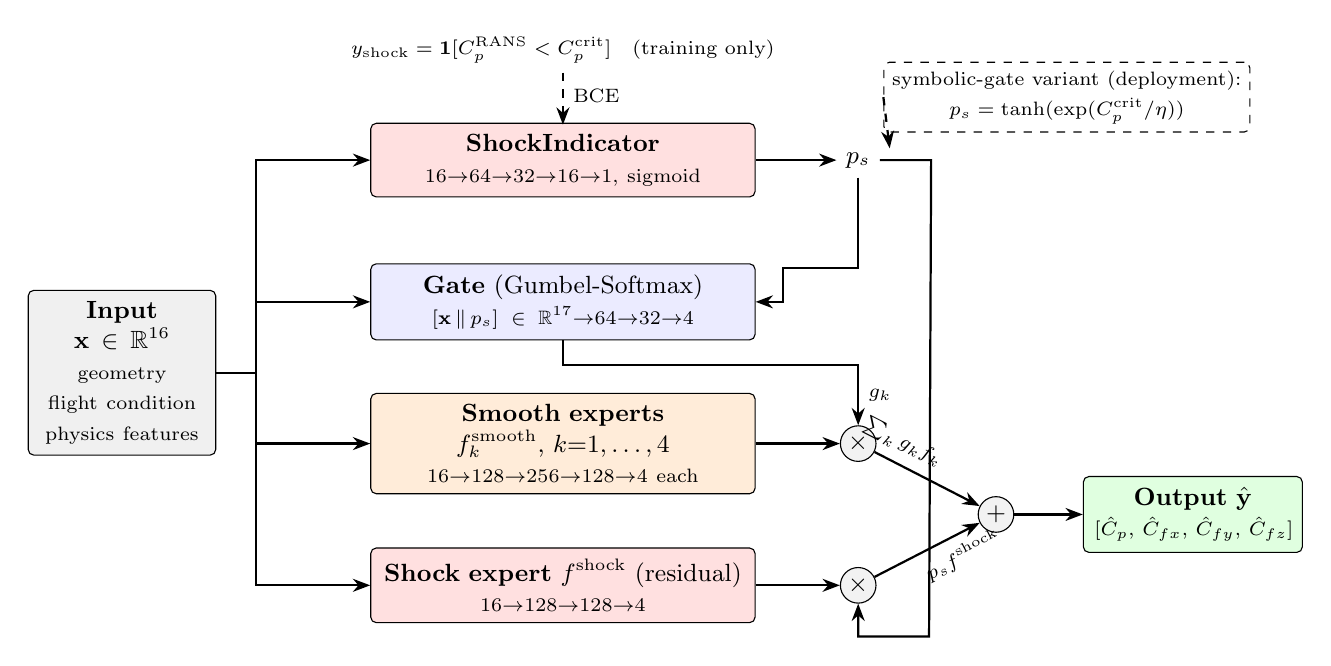
\begin{tikzpicture}[
  font=\small,
  blk/.style={draw, rounded corners=2pt, align=center,
              inner sep=4pt, text width=46mm},
  op/.style={draw, circle, inner sep=1.2pt, fill=gray!10},
  arrow/.style={-{Stealth[length=2.2mm]}, thick}
]
% Input
\node[blk, fill=gray!12, text width=21mm] (input) at (0,0)
  {\textbf{Input}\\ $\mathbf{x}\in\mathbb{R}^{16}$\\
  {\scriptsize geometry}\\
  {\scriptsize flight condition}\\
  {\scriptsize physics features}};

% Central column
\node[blk, fill=red!12] (si) at (5.6,2.7)
  {\textbf{ShockIndicator}\\
  {\scriptsize $16{\to}64{\to}32{\to}16{\to}1$, sigmoid}};
\node[blk, fill=blue!8] (gate) at (5.6,0.9)
  {\textbf{Gate} (Gumbel-Softmax)\\
  {\scriptsize $[\mathbf{x}\,\|\,p_s]\in\mathbb{R}^{17}{\to}64{\to}32{\to}4$}};
\node[blk, fill=orange!15] (e1) at (5.6,-0.9)
  {\textbf{Smooth experts} $f_k^{\mathrm{smooth}}$, $k{=}1,\dots,4$\\
  {\scriptsize $16{\to}128{\to}256{\to}128{\to}4$ each}};
\node[blk, fill=red!12] (se) at (5.6,-2.7)
  {\textbf{Shock expert} $f^{\mathrm{shock}}$ (residual)\\
  {\scriptsize $16{\to}128{\to}128{\to}4$}};

% Training-only supervision (dashed)
\node[align=center] (ysh) at (5.6,4.1)
  {\scriptsize $y_{\mathrm{shock}}=\mathbf{1}[C_p^{\mathrm{RANS}}<C_p^{\mathrm{crit}}]$
   \; (training only)};
\draw[-{Stealth[length=2.2mm]}, thick, dashed] (ysh)
  -- node[right, pos=0.45]{\scriptsize BCE} (5.6,3.15);

% Symbolic-gate deployment variant (dashed)
\node[draw, dashed, rounded corners=2pt, align=center, inner sep=3pt]
  (symnote) at (12.0,3.5)
  {\scriptsize symbolic-gate variant (deployment):\\
   \scriptsize $p_s=\tanh(\exp(C_p^{\mathrm{crit}}/\eta))$};
\draw[-{Stealth[length=2.2mm]}, thick, dashed] (symnote.west)
  -- (9.75,2.85);

% Operators and output
\node (ps) at (9.35,2.7) {$p_s$};
\node[op] (mult) at (9.35,-0.9) {$\times$};
\node[op] (mult2) at (9.35,-2.7) {$\times$};\node[op] (plus) at (11.1,-1.8) {$+$};
\node[blk, fill=green!12, text width=25mm] (out) at (13.6,-1.8)
  {\textbf{Output} $\hat{\mathbf{y}}$\\
  {\scriptsize $[\hat{C}_p,\,\hat{C}_{fx},\,\hat{C}_{fy},\,\hat{C}_{fz}]$}};

% Input fan-out
\draw[arrow] (input.east) -- ++(0.5,0) |- (si.west);
\draw[arrow] (input.east) -- ++(0.5,0) |- (gate.west);
\draw[arrow] (input.east) -- ++(0.5,0) |- (e1.west);
\draw[arrow] (input.east) -- ++(0.5,0) |- (se.west);

% Shock probability paths
\draw[arrow] (si.east) -- (ps);
\draw[arrow] (ps.south) -- ++(0,-1.15) -| ($(gate.east)+(0.35,0)$)
  -- node[above, pos=0.5]{} (gate.east);
\draw[arrow] (ps.east) -- ++(0.65,0) -- (10.25,-3.35) -- (9.35,-3.35)
  -- (mult2.south);

% Gate weights
\draw[arrow] (gate.south) -- (5.6,0.1) -- (9.35,0.1)
  -- node[right, pos=0.5]{\scriptsize $g_k$} (mult.north);

% Expert paths
\draw[arrow] (e1.east) -- (mult.west);
\draw[arrow] (se.east) -- (mult2.west);

% Combination
\draw[arrow] (mult) -- node[sloped, above, pos=0.18]{\scriptsize $\textstyle\sum_k g_k f_k$} (plus);
\draw[arrow] (mult2) -- node[sloped, below, pos=0.75]{\scriptsize $p_s f^{\mathrm{shock}}$} (plus);
\draw[arrow] (plus) -- (out);
\end{tikzpicture}
\caption{AeroSurrogate architecture (305\,753 parameters).  The
  ShockIndicator maps $\mathbf{x}$ to a shock probability $p_s$.  The
  gate routes the four smooth experts using both $\mathbf{x}$ and
  $p_s$; the shock expert contributes an additive residual scaled by
  $p_s$, providing an explicit discontinuity mechanism.  Dashed
  elements exist only at training time (BCE supervision) or in the
  symbolic-gate deployment variant.  At inference only $\mathbf{x}$
  is required---no CFD solver output.}
\label{fig:architecture}
\end{figure}

\subsection{ShockIndicator}
\label{sec:indicator}

The ShockIndicator is an MLP with layer sizes
$16\!\to\!64\!\to\!32\!\to\!16\!\to\!1$; every hidden layer applies
LayerNorm~\cite{Ba2016}, SiLU activation~\cite{Elfwing2018}, and
dropout (rate 0.1), and the final layer is linear:
\begin{equation}
  \mathrm{shock\_logit} = f_{\mathrm{SI}}(\mathbf{x};\theta_{\mathrm{SI}})
  \in \mathbb{R},
  \qquad
  p_s = \sigma(\mathrm{shock\_logit}) \in [0,1]
  \label{eq:indicator}
\end{equation}
It is supervised by the RANS-derived label $y_{\mathrm{shock}}$
through a binary cross-entropy term (Section~\ref{sec:loss}), so that
$p_s$ acquires the direct physical interpretation
$p_s \approx P(M_{\mathrm{local}} > 1)$.  Because the indicator is
trained end-to-end inside the surrogate, no separate pretraining stage
is needed, and the scalar $p_s$ serves simultaneously as (i)~an
input to the routing gate, (ii)~the multiplicative gain of the shock
expert, and (iii)~an interpretable shock-detection output in its own
right.

\subsection{Shock-gated Mixture of Experts}
\label{sec:moe}

The ShockGatedMoE comprises a gating network, $K=4$ smooth experts,
and one shock expert.  The \textbf{gate} receives the concatenation
$[\mathbf{x}\,\|\,p_s]\in\mathbb{R}^{17}$ and maps it through
$17\!\to\!64\!\to\!32\!\to\!4$ (LayerNorm + SiLU on hidden layers) to
$K$ routing logits $\mathbf{l}$, so that the routing decision is
informed by both the flight condition and the estimated shock state.
Each \textbf{smooth expert} is an MLP
$16\!\to\!128\!\to\!256\!\to\!128\!\to\!4$ (LayerNorm + SiLU +
dropout); the four experts specialise on smooth regime-dependent
loading patterns (e.g.\ subsonic attached flow, low-incidence
transonic flow, high-Mach conditions, high-incidence separated flow),
a specialisation that emerges from routing rather than explicit
labels~\cite{Jacobs1991,Shazeer2017}.  The \textbf{shock expert} is a
smaller MLP $16\!\to\!128\!\to\!128\!\to\!4$ whose output enters the
prediction as an additive residual scaled by $p_s$:
\begin{equation}
  \hat{\mathbf{y}} =
    \underbrace{\sum_{k=1}^{K} g_{k}(\mathbf{x}, p_s)\,
                f_{k}^{\mathrm{smooth}}(\mathbf{x})}_{\text{smooth MoE output}}
    \;+\;
    \underbrace{p_s\, f^{\mathrm{shock}}(\mathbf{x})}_{\text{shock residual}}
  \label{eq:forward}
\end{equation}

The shock residual is the key architectural innovation.  A smooth MLP
can only approximate a discontinuous function by smearing it, and
assigning one of the standard experts to shocked flow does not remove
this limitation---that expert would still need to be simultaneously
differentiable and sharply discontinuous.  The residual formulation
instead mirrors the physics: the total aerodynamic loading is
decomposed into a smooth background plus a shock perturbation.  In
subsonic flow $p_s\!\approx\!0$ and the correction vanishes
identically; inside the supersonic pocket $p_s\!\approx\!1$ and the
shock expert supplies the learned pressure-jump correction.  The
transition sharpness is inherited from the sigmoid of the
ShockIndicator rather than being limited by the smoothness of the
regression experts.

\subsection{Mach-gated Gumbel-Softmax routing}
\label{sec:gumbel}

Hard (argmax) expert selection would make the gradients of all
non-selected experts vanish and collapse training.  During training
the gate therefore uses the Gumbel-Softmax
relaxation~\cite{Jang2017,Maddison2017}, which provides
differentiable, near-one-hot routing as the temperature $\tau$ is
annealed:
\begin{equation}
  \mathbf{g} =
  \begin{cases}
    \mathrm{GumbelSoftmax}(\mathbf{l}/\tau) & \text{if } M > 0.75
      \quad \text{(transonic)}\\[2pt]
    \mathrm{softmax}(\mathbf{l}/\tau)       & \text{otherwise}
      \quad \text{(subsonic)}
  \end{cases}
  \label{eq:routing}
\end{equation}
with the exponential temperature schedule
\begin{equation}
  \tau(t) = \tau_{0}\left(\frac{\tau_{T}}{\tau_{0}}\right)^{t/T},
  \qquad \tau_{0}=1.0,\quad \tau_{T}=0.3,
  \label{eq:tau}
\end{equation}
where $t$ is the current epoch and $T$ the total number of epochs.
The freestream Mach number is recovered inside the forward pass by
denormalising the corresponding input feature with the stored scaler
statistics.  The stochastic Gumbel noise is deliberately applied
\emph{only to transonic points}: for subsonic points the $C_p$
distribution is smooth and unambiguous, and routing noise would merely
corrupt a clean signal, whereas in the transonic regime the shock
position varies between neighbouring flight conditions, so stochastic
routing acts as a form of data augmentation that improves expert
robustness.  The threshold $M=0.75$ is the conventional lower boundary
of the transonic regime.  At inference the gate uses a deterministic
softmax with the final temperature $\tau_T=0.3$, giving sharp but
noise-free routing.

\subsection{Normalisation and activation choices}
\label{sec:norm}

All hidden layers in AeroSurrogate use LayerNorm and SiLU, a
deliberate departure from the common BatchNorm + ReLU recipe.
BatchNorm computes batch statistics during training but applies
running averages at inference; with the strongly heterogeneous data
distribution across flight conditions this introduced a systematic
train/evaluation gap in early experiments.  LayerNorm normalises each
sample over its feature dimensions and therefore behaves identically
at training and inference, eliminating the gap entirely.  SiLU
($x\,\sigma(x)$)~\cite{Elfwing2018,Ramachandran2017} is smooth and
avoids the dead-neuron pathology that ReLU can exhibit in combination
with LayerNorm, and consistently outperformed ReLU-family activations
on this regression task.

\subsection{Loss function}
\label{sec:loss}

Training minimises a three-term objective:
\begin{equation}
  \mathcal{L} =
    \underbrace{\frac{1}{B}\sum_{i=1}^{B} w_i\,
      \|\hat{\mathbf{y}}_i - \mathbf{y}_i\|_{2}^{2}}_{\text{shock-weighted MSE}}
    \;+\; \lambda_{s}\,
    \underbrace{\mathrm{BCE}\bigl(\mathrm{shock\_logit},\,
      y_{\mathrm{shock}}\bigr)}_{\text{indicator supervision}}
    \;+\; \lambda_{\mathrm{lb}}\,
    \underbrace{K\sum_{k=1}^{K}\bar{g}_{k}^{2}}_{\text{load balance}}
  \label{eq:loss}
\end{equation}
with per-point weights
\begin{equation}
  w_i = 1 + \lambda_{\mathrm{sw}}\;y_{\mathrm{shock},i}\,
        \mathbf{1}\!\left[M_i > 0.75\right],
  \qquad
  \lambda_{s}=0.1,\quad \lambda_{\mathrm{lb}}=0.01,\quad
  \lambda_{\mathrm{sw}}=5.0
  \label{eq:weights}
\end{equation}
The \emph{shock-weighted MSE} assigns $6\times$ loss weight to points
that carry a positive shock label \emph{and} lie in the transonic
range, focusing capacity on the shock region where the smoothing
pathology is most damaging; subsonic points with spurious
$C_p<C_p^{\mathrm{crit}}$ labels (physically ambiguous at low Mach)
retain unit weight.  The \emph{BCE term} supervises the
ShockIndicator with positive-class weight 5.0 to compensate for label
imbalance ($\approx$14--19\% positives).  The \emph{load-balance
term}, in the style of Switch-Transformer auxiliary
losses~\cite{Shazeer2017,Fedus2022}, penalises the squared
batch-averaged gate weights $\bar{g}_k$ (it attains its minimum of
1.0 under perfectly uniform routing), preventing gate collapse onto a
single expert.

\subsection{Training procedure}
\label{sec:training}

The complete workflow consists of four steps
(Figure~\ref{fig:pipeline}): (1)~preprocessing, which computes the
derived features, fits the z-score scalers, and materialises the
train/test arrays; (2)~end-to-end training of AeroSurrogate with the
neural ShockIndicator gate; (3)~symbolic distillation of the shock
criterion with PySR (Section~\ref{sec:sr}); and (4)~retraining of the
MoE with the frozen symbolic gate.  In step~4 the BCE term of
Eq.~(\ref{eq:loss}) is dropped, since the shock probability is
supplied by the fixed algebraic formula rather than by a trainable
network.

\begin{figure}[ht]
\centering
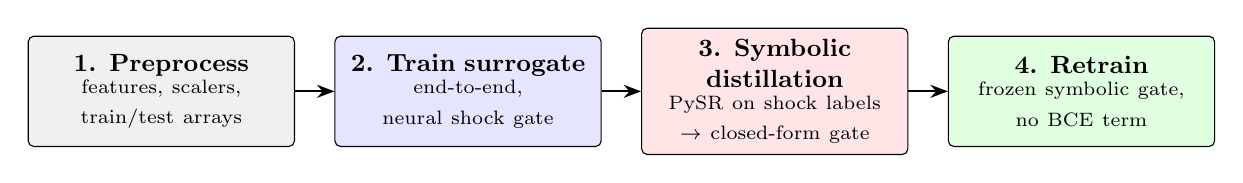
\begin{tikzpicture}[
  font=\small,
  stepblk/.style={draw, rounded corners=2pt, align=center,
               minimum height=14mm, inner sep=4pt, text width=31mm},
  arrow/.style={-{Stealth[length=2.2mm]}, thick}
]
\node[stepblk, fill=gray!12]  (s1) {\textbf{1. Preprocess}\\
  {\scriptsize features, scalers,\\ train/test arrays}};
\node[stepblk, fill=blue!10, right=5mm of s1]  (s2) {\textbf{2. Train surrogate}\\
  {\scriptsize end-to-end,\\ neural shock gate}};
\node[stepblk, fill=red!10, right=5mm of s2]  (s3) {\textbf{3. Symbolic distillation}\\
  {\scriptsize PySR on shock labels\\ $\to$ closed-form gate}};
\node[stepblk, fill=green!12, right=5mm of s3]  (s4) {\textbf{4. Retrain}\\
  {\scriptsize frozen symbolic gate,\\ no BCE term}};
\draw[arrow] (s1) -- (s2);
\draw[arrow] (s2) -- (s3);
\draw[arrow] (s3) -- (s4);
\end{tikzpicture}
\caption{Four-step training pipeline.  Steps 2 and 4 run on GPU;
  step 3 runs the PySR evolutionary search.}
\label{fig:pipeline}
\end{figure}

Optimisation uses Adam ($\beta_1=0.9$, $\beta_2=0.999$) with learning
rate $10^{-3}$, weight decay $10^{-5}$, gradient-norm clipping at
1.0, batch size 256, and up to 200 epochs with early stopping
(patience 5, tolerance $10^{-4}$) monitored on plain validation MSE
(without shock weighting or auxiliary terms), so that checkpoint
selection is not biased by the training-time reweighting.
Table~\ref{tab:arch} summarises the architecture and training
hyperparameters.

\begin{table}[ht]
\centering
\caption{Architecture and training hyperparameters of AeroSurrogate
  (305\,753 parameters in total).}
\label{tab:arch}
\begin{tabular}{lll}
\toprule
\textbf{Component} & \textbf{Parameter} & \textbf{Value} \\
\midrule
ShockIndicator & Layers & $16{\to}64{\to}32{\to}16{\to}1$ \\
               & Hidden blocks & LayerNorm + SiLU + Dropout(0.1) \\
\midrule
Gate           & Layers & $17{\to}64{\to}32{\to}4$ \\
               & Routing & Gumbel-Softmax, $\tau: 1.0 \to 0.3$ (exp.) \\
               & Transonic threshold & $M > 0.75$ \\
\midrule
Smooth experts & Number $K$ & 4 \\
               & Layers (each) & $16{\to}128{\to}256{\to}128{\to}4$ \\
\midrule
Shock expert   & Layers & $16{\to}128{\to}128{\to}4$ \\
               & Coupling & residual, scaled by $p_s$ \\
\midrule
Loss           & $\lambda_{s}$ / $\lambda_{\mathrm{lb}}$ / $\lambda_{\mathrm{sw}}$ & 0.1 / 0.01 / 5.0 \\
               & BCE positive-class weight & 5.0 \\
\midrule
Optimisation   & Optimiser & Adam ($\beta_1{=}0.9$, $\beta_2{=}0.999$) \\
               & Learning rate / weight decay & $10^{-3}$ / $10^{-5}$ \\
               & Gradient clipping & $\|\nabla\|_2 \le 1.0$ \\
               & Batch size / epochs & 256 / 200 (early stopping) \\
\bottomrule
\end{tabular}
\end{table}

\subsection{Inference pipeline}
\label{sec:inference}

At inference, no CFD solver output is required.  The deployed model
consumes three sources only: the surface mesh nodes
$(x,y,z,n_x,n_y,n_z)$, available directly from the CAD or mesh file;
the flight condition $(M,\alpha,\Pi)$, taken from the test matrix or
flight envelope; and two one-time training artefacts, namely the
z-score statistics and the chord/span bounds fitted once on the
training mesh.  Prediction then proceeds in four steps:
\begin{enumerate}
  \item \emph{Analytical feature construction}: the five physics
        features are evaluated from the closed-form isentropic
        relations of Eqs.~(\ref{eq:derived1})--(\ref{eq:cpcrit}), and
        the two geometry features $x_{\mathrm{norm}}$ and $\eta$ are
        linear rescalings of the mesh coordinates using the stored
        bounds, yielding $\mathbf{x}\in\mathbb{R}^{16}$ with no solver
        call.
  \item \emph{Normalisation} of $\mathbf{x}$ with the stored training
        statistics.
  \item \emph{A single forward pass} through AeroSurrogate,
        Eq.~(\ref{eq:forward}), producing the four normalised
        coefficients and, as a by-product, the shock probability
        $p_s$ and the gate weights.
  \item \emph{Denormalisation} of
        $[\hat{C}_p,\hat{C}_{fx},\hat{C}_{fy},\hat{C}_{fz}]$ to
        physical units.
\end{enumerate}
In the symbolic-gate variant (Section~\ref{sec:sr}), step~3 replaces
the ShockIndicator by the closed-form expression
$\tanh(\exp(C_p^{\mathrm{crit}}/\eta))$, reducing the entire
shock-routing mechanism to elementary scalar arithmetic---no neural
shock detection network is evaluated at all.  The complete
pipeline---feature construction plus network forward pass---operates
on millisecond time scales per surface point batch, compared with
$\mathcal{O}(10^{3}$--$10^{4})$ CPU-hours for a RANS solution of a
single flight condition, while requiring only surface-level inputs
that are equally available in experimental or flight-test contexts.

% ================================================================
\section{SYMBOLIC DISTILLATION OF THE SHOCK CRITERION}
\label{sec:sr}
% ================================================================

After the neural surrogate is trained, the shock-detection function
is distilled into a closed-form algebraic expression using
PySR~\cite{Cranmer2020}.  This serves three purposes:
(i)~\emph{interpretability}---a human-readable equation for the shock
criterion; (ii)~\emph{physical validation}---if the recovered
equation reproduces known shock physics, the network has learned
genuine aerodynamics rather than spurious correlations; and
(iii)~\emph{lightweight deployment}---the symbolic gate requires only
elementary arithmetic, no neural inference.

\subsection{Setup}

The SR stage regresses the \emph{hard physics label}
$y_{\mathrm{shock}}\in\{0,1\}$ of Eq.~(\ref{eq:labels})---not the
soft output of the neural ShockIndicator---on a subset of nine
physically meaningful features:
\begin{equation}
  \mathbf{x}_{\mathrm{sr}} = [\,M,\;\alpha,\;x_{\mathrm{norm}},\;
  \eta,\; n_{z},\; C_{p}^{\mathrm{crit}},\; q_{\mathrm{dyn}},\;
  \mathrm{AoA}_{\sin},\; L_{\mathrm{factor}}\,]
  \label{eq:srfeatures}
\end{equation}
Raw geometric coordinates $(x,y,z)$ and the normal components
$(n_x,n_y)$ are excluded to bias the search toward conditions based
on flow physics and aerodynamically meaningful coordinates rather
than absolute surface location.  PySR performs a multi-objective
evolutionary search (200 iterations, 50\,000 training samples) over
expression trees built from the operator set
$\{+,\,-,\,\times,\,\div,\,\exp,\,\tanh\}$, minimising the MSE
penalised by expression complexity (node count), and returns a Pareto
front of candidate expressions.  A RandomForest classifier is trained
in parallel on the same features to provide a model-agnostic feature
importance ranking.

\subsection{Results of the symbolic search}
\label{sec:srresults}

Figure~\ref{fig:importance} reports the RandomForest feature
importances.  Chord-wise and span-wise position dominate, followed by
the Mach number and its derived quantities.  This ranking is
physically consistent: on a transonic transport wing the shock sits
at a characteristic chord fraction ($x/c \approx 0.3$--$0.6$) over
the mid-span region, and its occurrence is then modulated by the
freestream Mach number.  This analysis motivated the inclusion of
$x_{\mathrm{norm}}$ and $\eta$ in the 16-feature input vector.

\begin{figure}[ht]
\centering
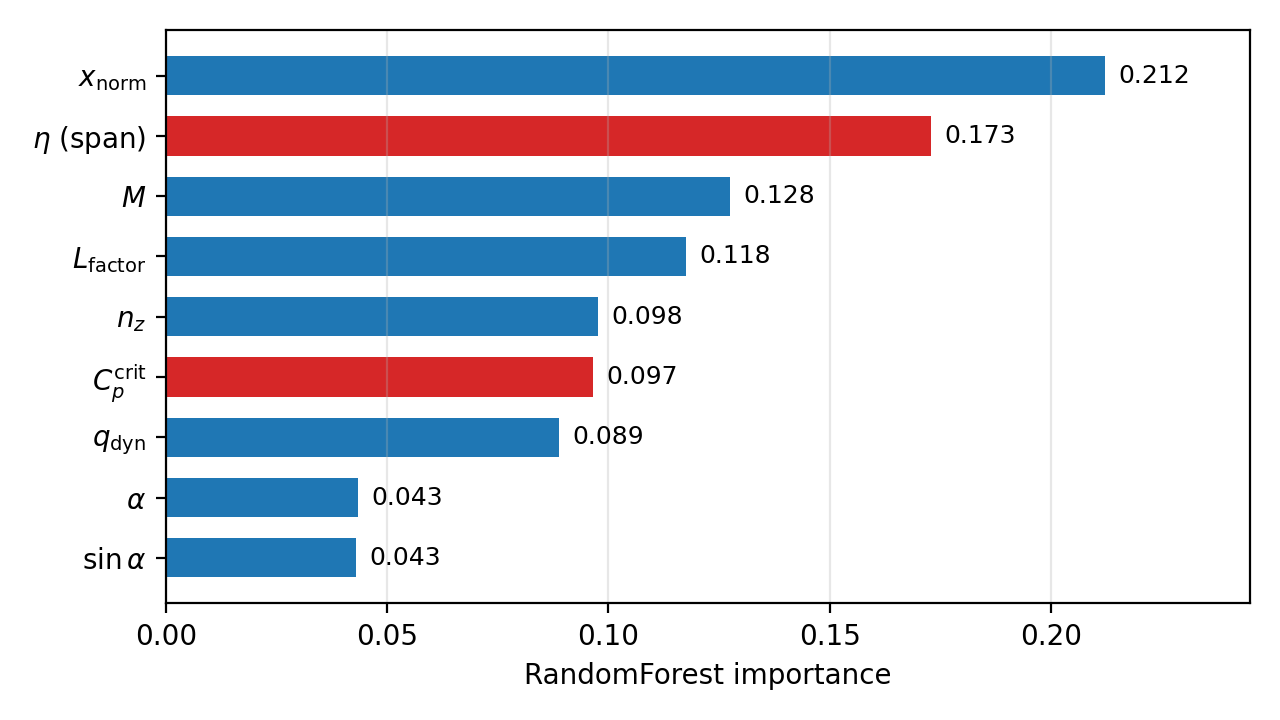
\includegraphics[width=0.75\textwidth]{figures/feature_importance.png}
\caption{RandomForest feature importances for shock classification,
  trained on the physics labels of Eq.~(\ref{eq:labels}).  Red bars
  mark the two variables that appear in the selected symbolic
  expression.}
\label{fig:importance}
\end{figure}

From the Pareto front (Figure~\ref{fig:pareto};
Table~\ref{tab:pareto} lists the leading expressions), the
complexity-5 expression with the highest score is selected:
\begin{equation}
  \boxed{\;\hat{y}_{\mathrm{shock}}^{\mathrm{SR}}
  = \tanh\!\left(\exp\!\left(
      \frac{C_{p}^{\mathrm{crit}}(M)}{\eta}\right)\right)\;}
  \label{eq:srdiscovered}
\end{equation}

\begin{table}[ht]
\centering
\caption{Top of the PySR Pareto front (score balances accuracy gain
  against complexity increase; complexity = expression-tree node
  count).}
\label{tab:pareto}
\begin{tabular}{clc}
\toprule
\textbf{Complexity} & \textbf{Expression} & \textbf{Score} \\
\midrule
5 & $\tanh(\exp(C_p^{\mathrm{crit}} / \eta))$ & \textbf{0.0433} \\
4 & $\exp(C_p^{\mathrm{crit}} / \eta)$ & 0.0422 \\
8 & $\exp(2\,C_p^{\mathrm{crit}} / (\eta + 0.1799))$ & 0.0331 \\
6 & $\exp(C_p^{\mathrm{crit}} / \eta + C_p^{\mathrm{crit}})$ & 0.0293 \\
\bottomrule
\end{tabular}
\end{table}

\begin{figure}[ht]
\centering
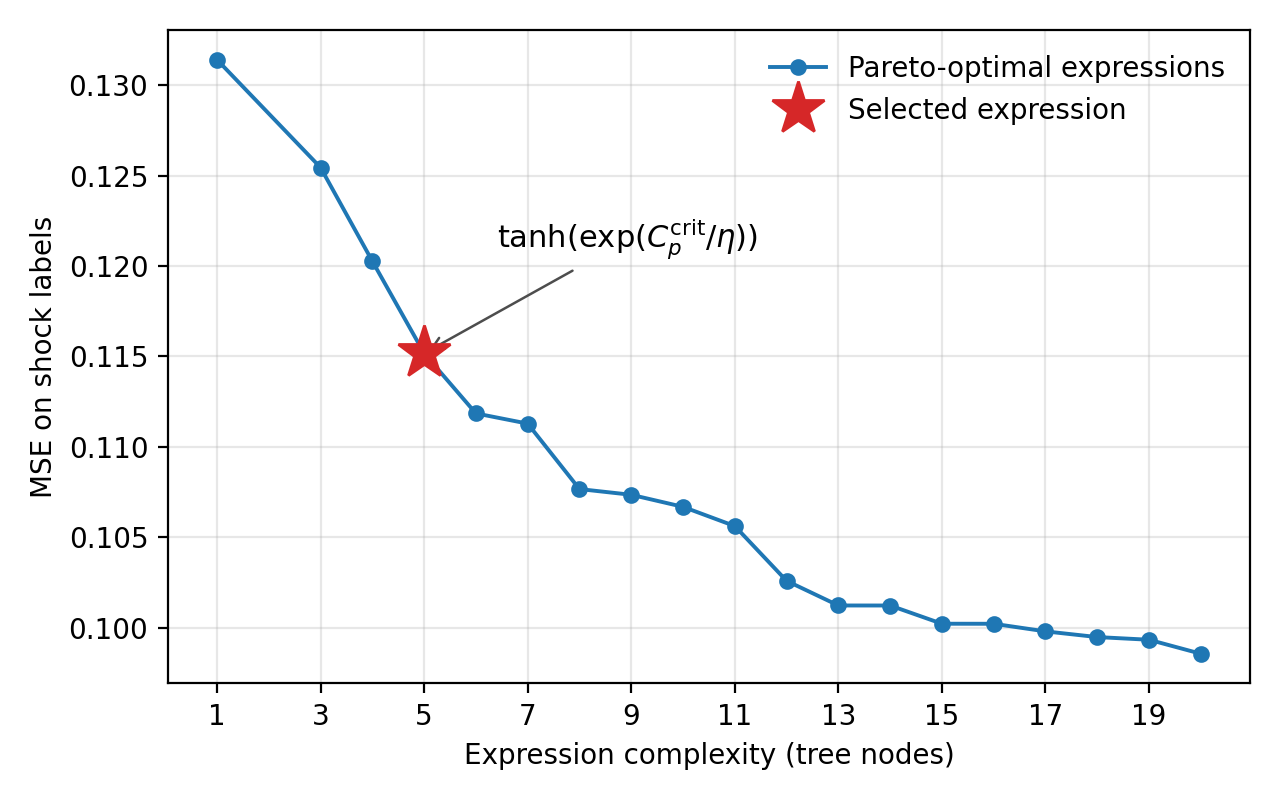
\includegraphics[width=0.72\textwidth]{figures/sr_pareto_front.png}
\caption{PySR Pareto front: MSE on the shock labels versus expression
  complexity.  The selected complexity-5 expression (star) sits at
  the elbow of the front, where accuracy gains begin to saturate
  relative to the added complexity.}
\label{fig:pareto}
\end{figure}

The expression admits a direct physical reading.  Since
$C_{p}^{\mathrm{crit}}(M)<0$ (the sonic condition always corresponds
to suction) and $\eta\in(0,1]$, the argument
$C_{p}^{\mathrm{crit}}/\eta$ is a Mach-dependent negative quantity
amplified toward the wing root.  Near the root the large-magnitude
negative argument drives $\exp(\cdot)\to 0$ and hence
$\hat{y}^{\mathrm{SR}}_{\mathrm{shock}}\to 0$---the inboard wing,
where the flow remains well attached under typical conditions.
Moving outboard, and as increasing Mach makes
$C_{p}^{\mathrm{crit}}$ less negative, the argument grows,
$\exp(\cdot)$ increases, and the predicted shock probability rises
over the mid-span region where transonic shocks typically form.  The
formula thus couples the two dominant factors identified
independently by the feature-importance analysis: proximity to the
sonic threshold (through $C_{p}^{\mathrm{crit}}$, a function of Mach
only) and span-wise station.  Figure~\ref{fig:symmap} maps the
expression over the $(M,\eta)$ plane: the iso-probability contours
sweep toward lower span stations as the Mach number increases,
reproducing the outboard growth and inboard extension of the
supersonic region with Mach that is characteristic of swept
transonic wings.  On the validation set the symbolic sensor achieves
an AUC-ROC of 0.6727 against the RANS-derived shock labels---notable
discrimination for a two-variable, five-node formula evaluated
pointwise with no access to the pressure field.

\begin{figure}[ht]
\centering
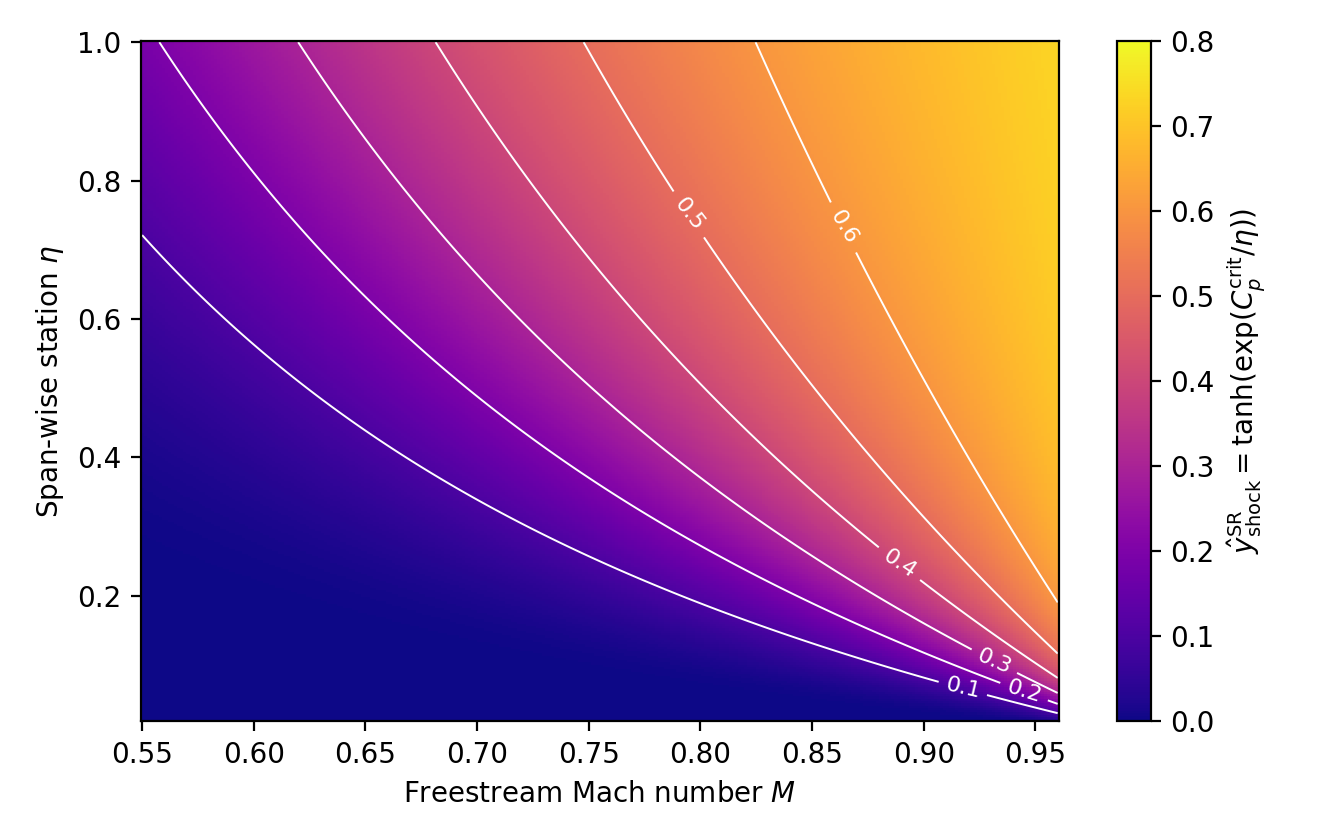
\includegraphics[width=0.7\textwidth]{figures/symbolic_sensor_map.png}
\caption{Shock probability predicted by the symbolic sensor of
  Eq.~(\ref{eq:srdiscovered}) over the Mach--span plane.  The sensor
  activates with increasing Mach and toward outboard span stations,
  consistent with the feature importances of
  Figure~\ref{fig:importance}.}
\label{fig:symmap}
\end{figure}

\subsection{Retraining with the frozen symbolic gate}
\label{sec:symgate}

The symbolic expression is an approximation of the neural
ShockIndicator, so simply substituting it at inference would create a
mismatch between the routing statistics seen during training and
deployment.  Instead, the surrogate is \emph{retrained} (step~4 of
Figure~\ref{fig:pipeline}) with the symbolic formula frozen as the
shock-probability source: the smooth experts, shock expert, and gate
adapt to the algebraic routing signal, and the BCE term is removed
from the loss.  The deployed model therefore uses the interpretable
formula exactly as trained, with no train/inference discrepancy.  As
shown in Section~\ref{sec:results}, this substitution is lossless in
terms of aerodynamic accuracy.

% ================================================================
\section{RESULTS AND DISCUSSION}
\label{sec:results}
% ================================================================

\subsection{Aerodynamic coefficient prediction}

Table~\ref{tab:results} reports the coefficient-of-determination
scores on the held-out test sample of 4\,068\,074 surface points,
for both the neural-gate model (step~2) and the symbolic-gate model
(step~4).  The surrogate achieves $R^{2}=0.9506$ for the pressure
coefficient and $R^{2}\approx 0.85$ for the three skin-friction
components, all three of which remain above $R^{2}=0.847$.
Aggregate error metrics for the symbolic-gate model are MSE
$=0.1228$, RMSE $=0.3504$, and MAE $=0.1612$ in normalised target
space.

The gap between pressure and friction accuracy deserves a physical
reading, since it is structural rather than incidental.  The surface
pressure is imposed predominantly by the outer, essentially inviscid
flow; it is therefore a direct---and largely local---function of the
geometry and flight condition that constitute the input vector.  The
skin friction, in contrast, is a wall-gradient quantity, proportional
to the wall-normal velocity gradient at the base of the boundary
layer: its magnitude is two to three orders smaller than the pressure
loading, and its local value encodes the upstream history of the
boundary layer---transition (fixed at 10\% chord in the database),
pressure-gradient history, and incipient separation---non-local
information that a point-wise input vector cannot fully represent.
The lateral and vertical components $C_{fy}$ and $C_{fz}$ are further
penalised because they are projections of the shear-stress vector
that change sign with local surface orientation and cross-flow
direction, so their distributions are centred near zero over large
portions of the airframe and the $R^{2}$ statistic becomes
intrinsically more demanding.  Finally, the RANS friction fields are
themselves the least reliable solver output at the extreme
incidences included in the envelope, where convergence
degrades~\cite{Peter2025}, so part of the residual is label noise
rather than model error.  The ranking observed here---$C_p$ best,
then the friction components---matches the reference results for
this database, where every regressor evaluated by
ONERA exhibits the same ordering, with friction $R^{2}$ scores
systematically below the pressure score and worst-case relative
errors on $C_{fy}$ and $C_{fz}$ up to twice those of
$C_p$~\cite{Peter2025}.

\begin{table}[ht]
\centering
\caption{Prediction accuracy on the held-out test sample
  (4\,068\,074 surface points).  The symbolic-gate model replaces the
  neural ShockIndicator with the closed-form expression of
  Eq.~(\ref{eq:srdiscovered}).}
\label{tab:results}
\begin{tabular}{lcccc}
\toprule
\textbf{Model} & $R^{2}(C_{p})$ & $R^{2}(C_{fx})$
               & $R^{2}(C_{fy})$ & $R^{2}(C_{fz})$ \\
\midrule
AeroSurrogate (neural gate)   & 0.9506 & 0.8508 & 0.8475 & 0.8557 \\
AeroSurrogate (symbolic gate) & 0.9506 & 0.8508 & 0.8475 & 0.8557 \\
\bottomrule
\end{tabular}
\end{table}

The central observation of Table~\ref{tab:results} is that the neural
and symbolic gates achieve \emph{identical} scores to four decimal
places.  The learned shock-detection function of the neural
ShockIndicator can be replaced by the five-node algebraic expression
of Eq.~(\ref{eq:srdiscovered}) without any measurable degradation of
the downstream aerodynamic prediction.  This is a strong data-driven
validation of the symbolic distillation: the routing information the
MoE actually exploits is fully captured by the two physical variables
$C_p^{\mathrm{crit}}(M)$ and $\eta$.

Figure~\ref{fig:parity} shows parity plots for the four coefficients
over the test sample.  The $C_p$ cloud is tight around the identity
line across its full range, including the strong-suction tail
generated by the shock-side suction peaks; the friction components
show the wider but unbiased scatter consistent with their lower
$R^2$.

\begin{figure}[ht]
\centering
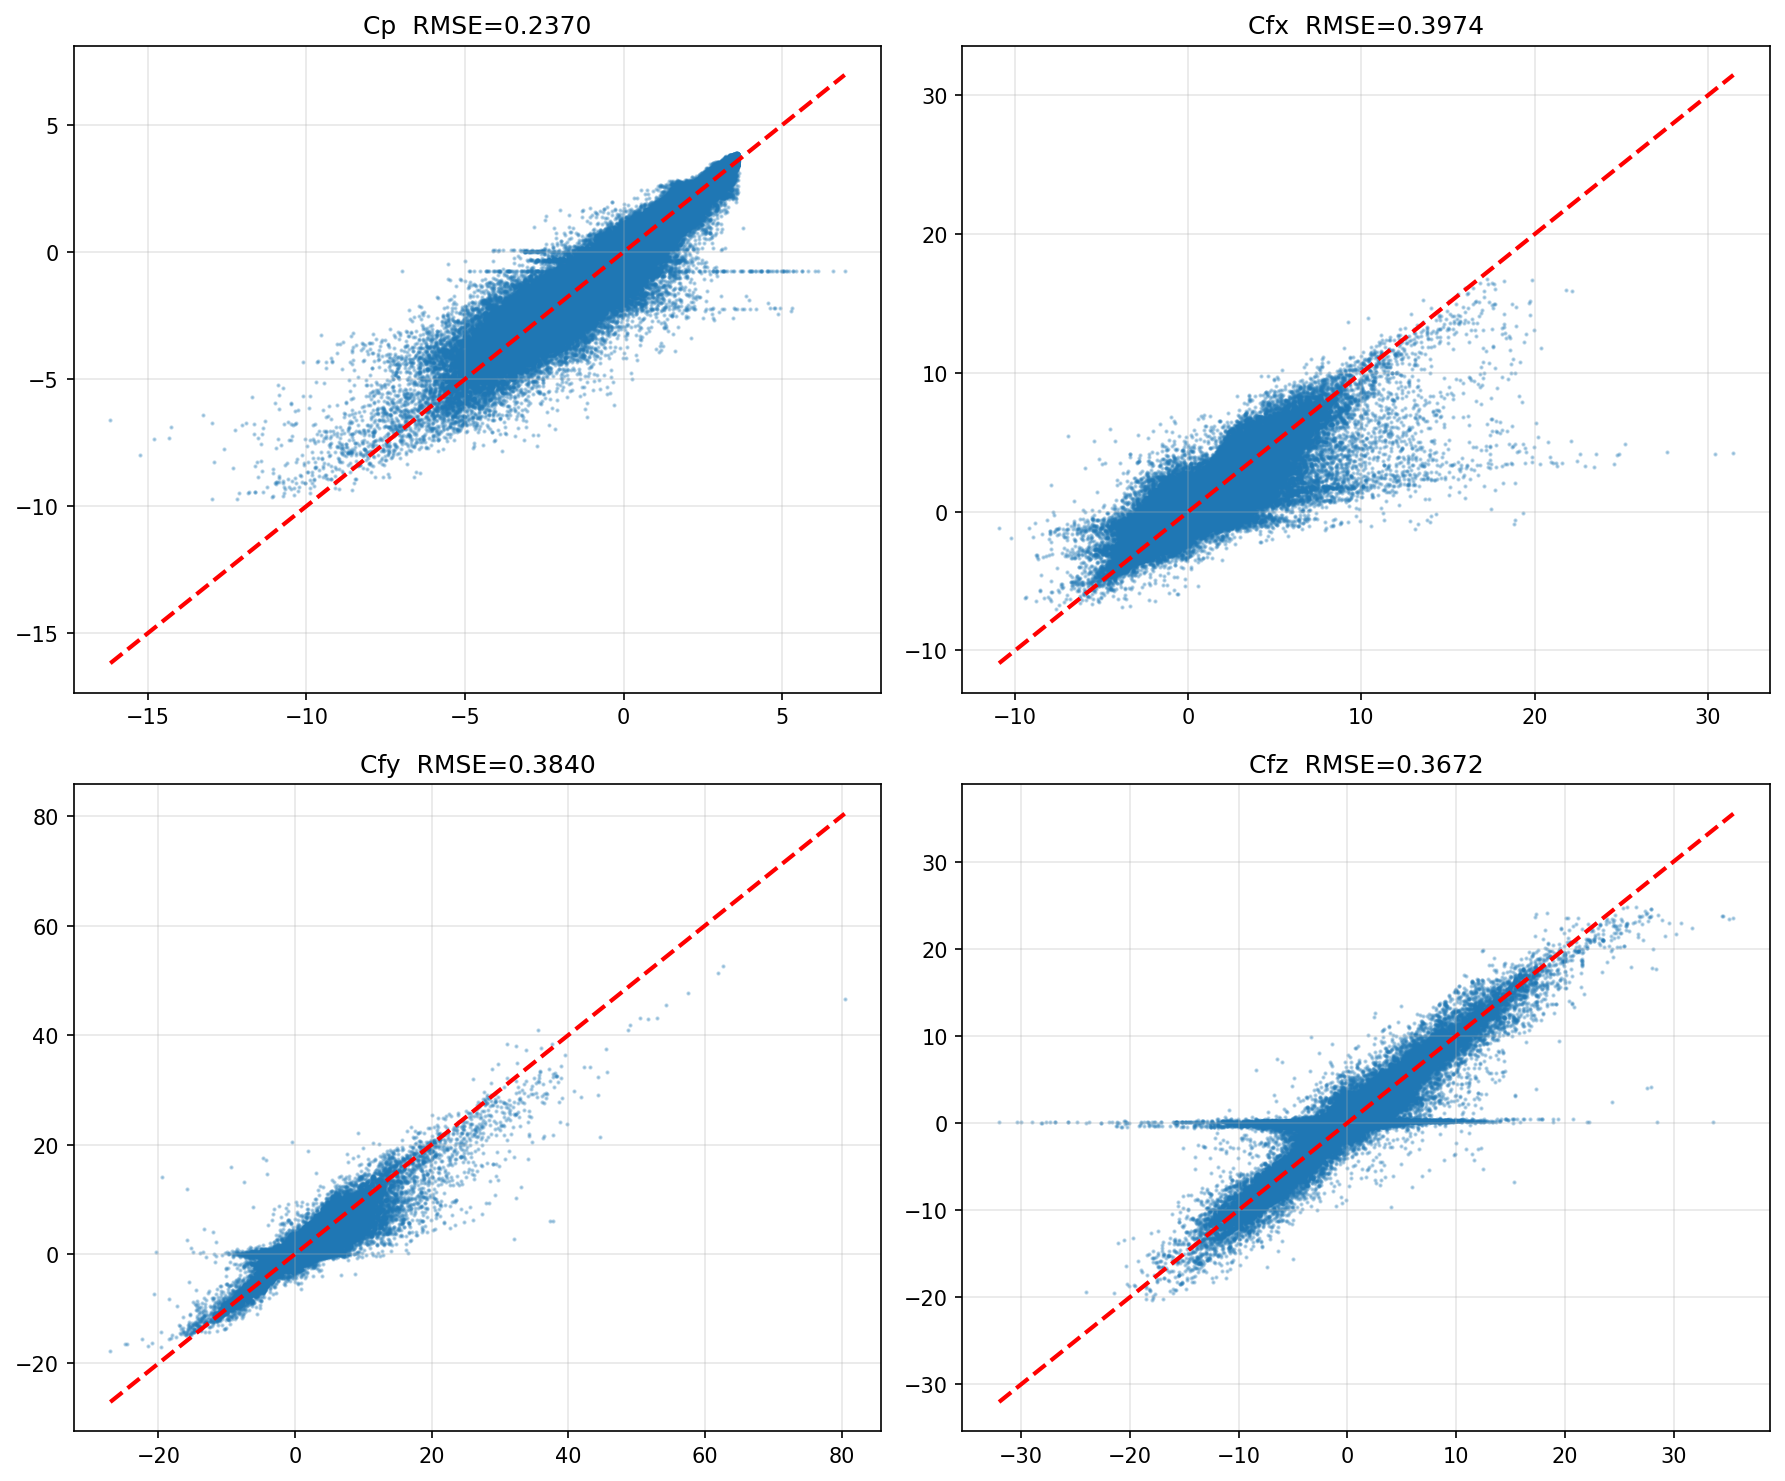
\includegraphics[width=0.92\textwidth]{figures/parity_plots.png}
\caption{Parity plots (predicted vs.\ RANS) for $C_p$, $C_{fx}$,
  $C_{fy}$ and $C_{fz}$ on the held-out test sample, symbolic-gate
  model.  The dashed red line is the identity.}
\label{fig:parity}
\end{figure}

\subsection{Full-aircraft surface fields}

Figures~\ref{fig:cond0}--\ref{fig:cond130} compare the RANS reference
fields, the surrogate prediction (symbolic gate), and the point-wise
relative error for all four surface coefficients
$[C_p, C_{fx}, C_{fy}, C_{fz}]$, on both the lower and upper aircraft
surfaces, for six held-out flight conditions spanning the envelope:
subsonic at negative incidence ($M{=}0.30$, $\alpha{=}-6^{\circ}$),
high-subsonic at strong negative incidence
($M{=}0.70$, $\alpha{=}-10^{\circ}$), transonic cruise
($M{=}0.80$, $\alpha{=}0^{\circ}$), transonic at moderate incidence
($M{=}0.84$, $\alpha{=}5^{\circ}$), high-transonic
($M{=}0.86$, $\alpha{=}0^{\circ}$), and a high-Mach, high-incidence
condition ($M{=}0.90$, $\alpha{=}6^{\circ}$).  In each figure the top
row shows
the CFD truth, the middle row the AeroSurrogate prediction, and the
bottom row the point-wise relative error.

The predicted fields reproduce the characteristic structure of each
regime.  In the subsonic case (Figure~\ref{fig:cond0}) the smooth
pressure distribution and the loading redistribution toward the lower
surface induced by the negative incidence are captured without
spurious oscillations.  At $M{=}0.70$, $\alpha{=}-10^{\circ}$
(Figure~\ref{fig:cond26}) the strong lower-surface suction and the
leading-edge pressure peaks of the inverted loading are correctly
reproduced.  At transonic cruise (Figure~\ref{fig:cond52}) the
upper-wing supersonic plateau and its terminating shock appear at the
correct chord-wise and span-wise station, and the associated
skin-friction signature in $C_{fx}$ is recovered.  As Mach and
incidence increase (Figures~\ref{fig:cond81}--\ref{fig:cond130}) the
shock strengthens, extends outboard, and moves aft; the surrogate
tracks this displacement, including the intensified suction levels
of the $M{=}0.90$, $\alpha{=}6^{\circ}$ case, among the most
demanding conditions shown.

The relative-error maps should be read with the metric's definition
in mind: the error is normalised by the local magnitude of the true
coefficient, so it saturates wherever that coefficient crosses zero.
The extended red patches on the fuselage in the $C_{fy}$ and
$C_{fz}$ panels arise precisely there---the true lateral and vertical
friction components are near zero over most of the fuselage---and
therefore correspond to negligible absolute errors, consistent with
the global $R^{2}$ scores of Table~\ref{tab:results} and the parity
plots of Figure~\ref{fig:parity}.  For $C_p$ the relative error is
low over most of the wetted surface and concentrates in narrow bands
along the shock front, where a small shift of the predicted shock
position produces locally large but physically benign discrepancies,
and along the $C_p{=}0$ isolines.  Among the friction components,
$C_{fx}$ shows the cleanest relative-error map, in line with its
larger characteristic magnitude.

\begin{figure}[H]
\centering
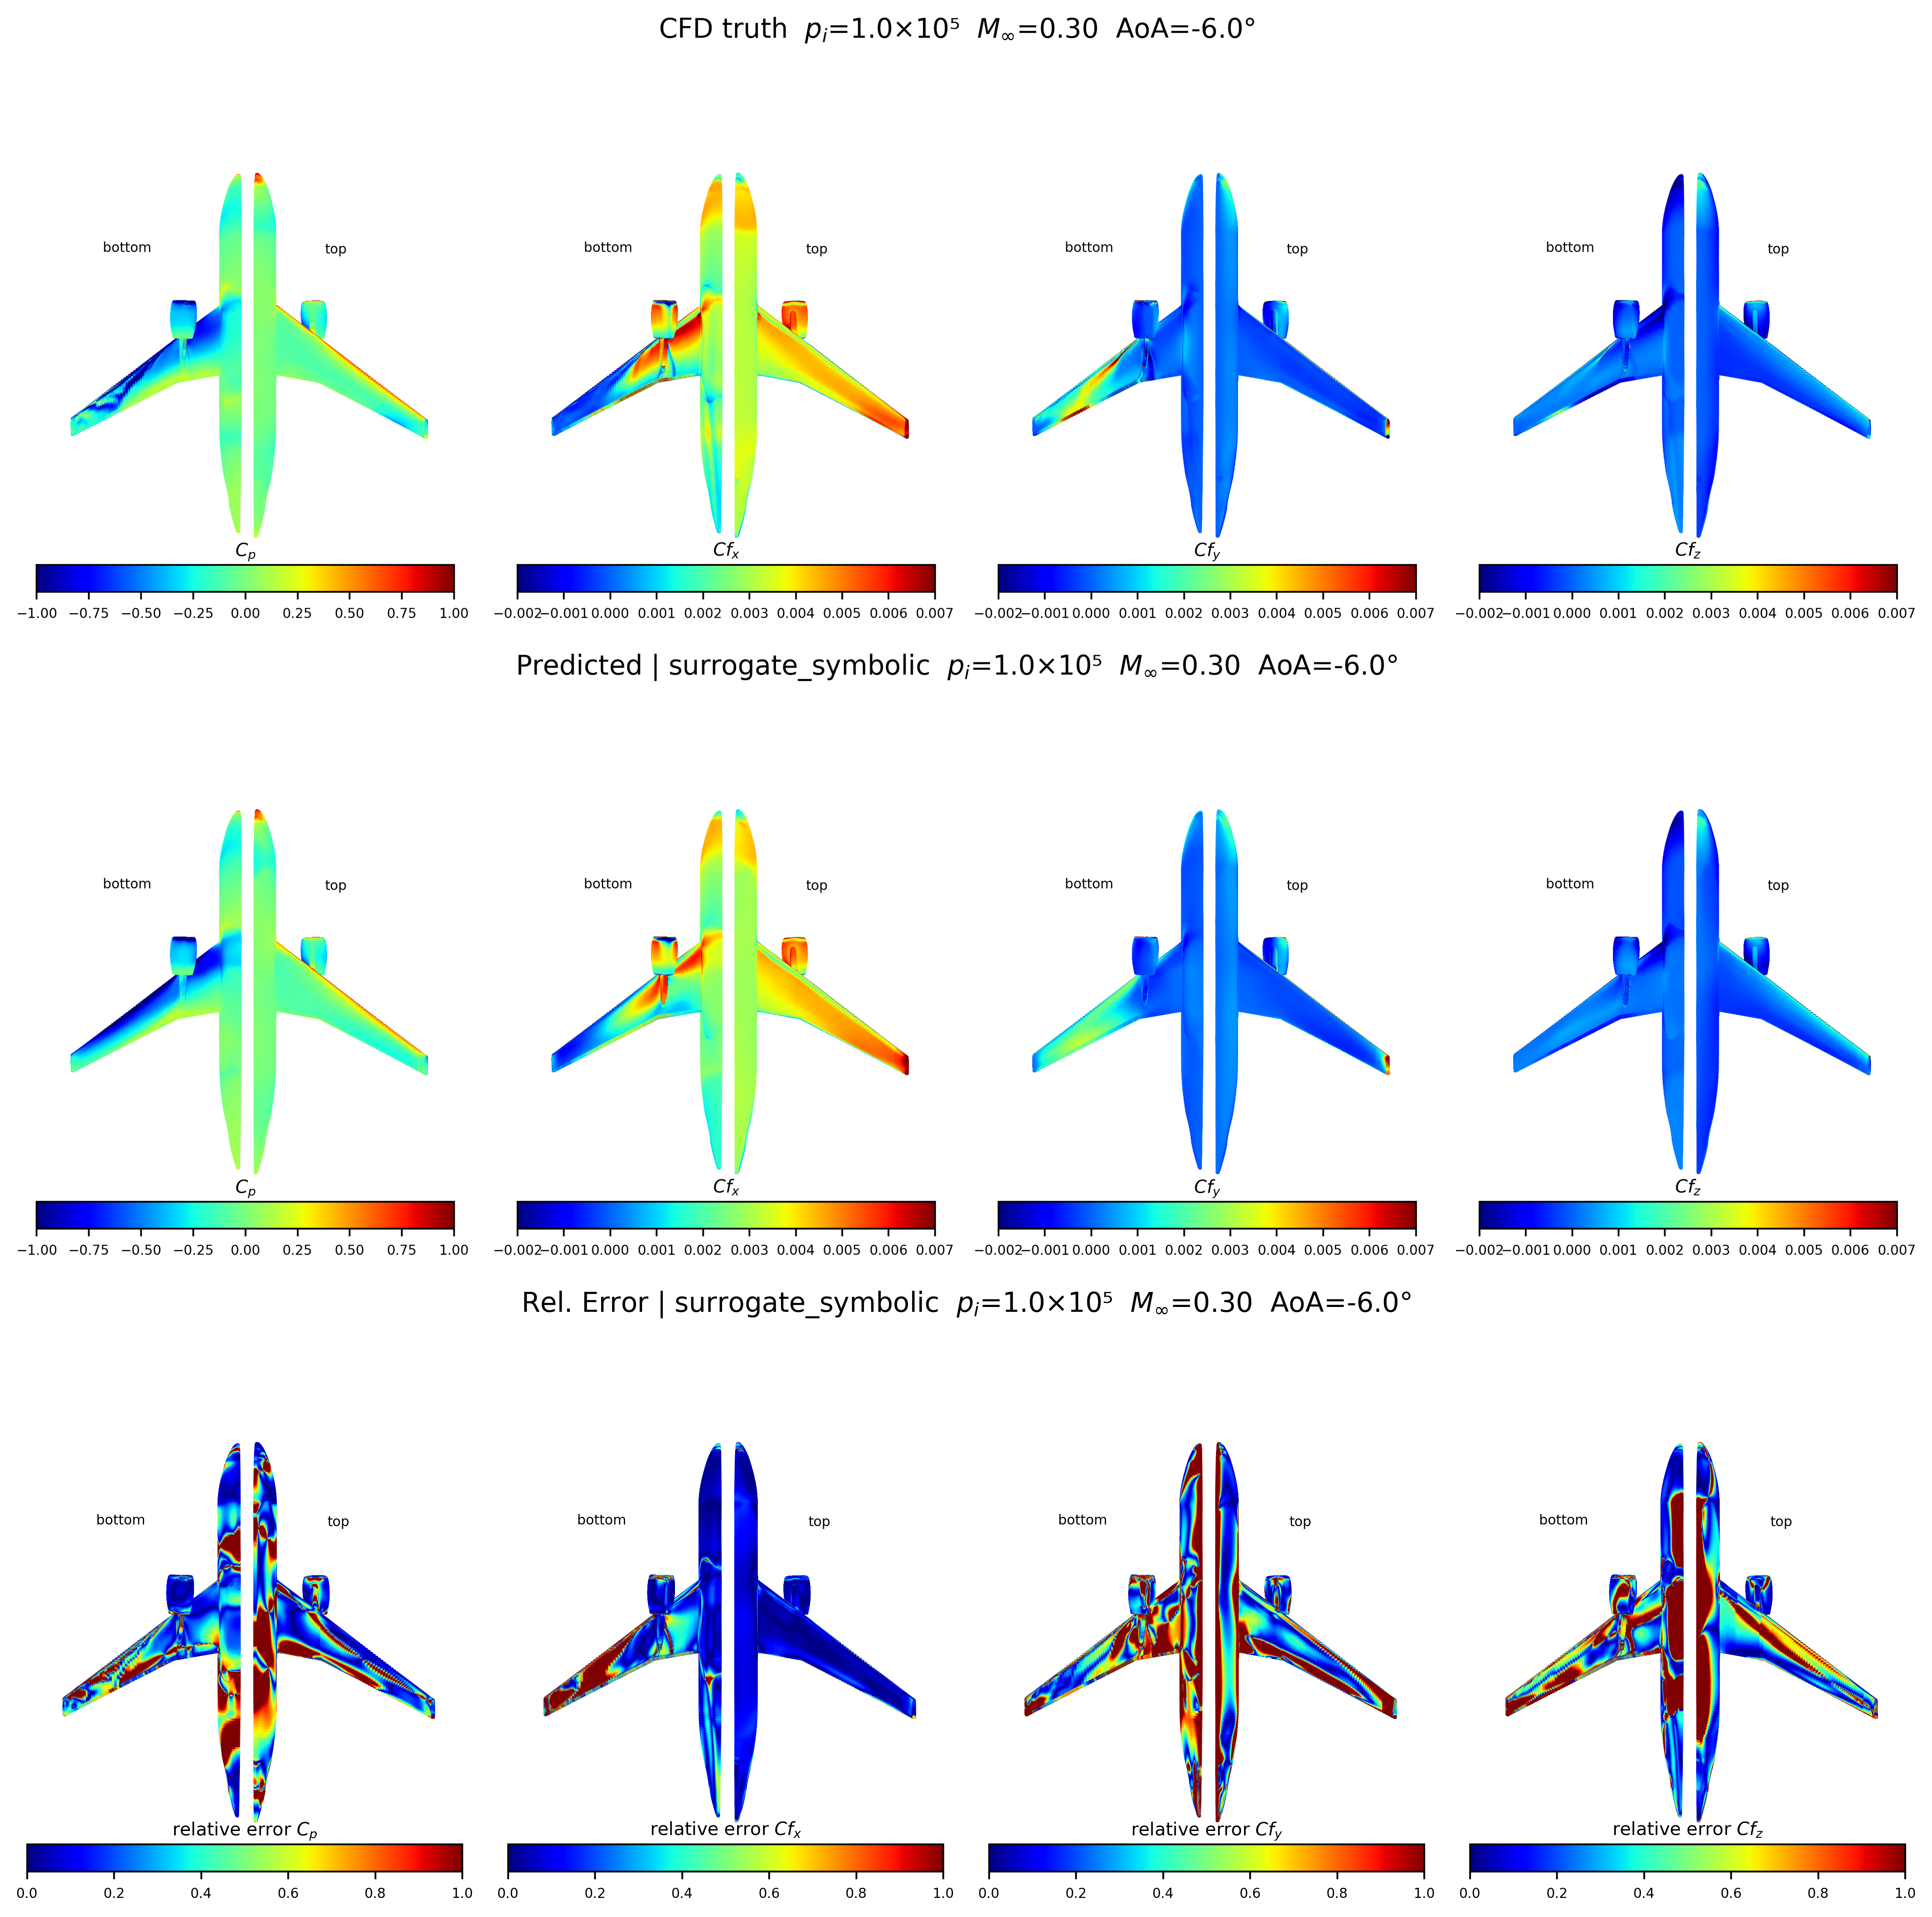
\includegraphics[width=0.88\textwidth]{figures/surface_fields_cond0.png}
\caption{Subsonic, negative incidence ($M{=}0.30$,
  $\alpha{=}-6^{\circ}$, $\Pi{=}1.0{\times}10^{5}$): CFD reference
  (top), AeroSurrogate prediction (middle) and point-wise relative
  error (bottom) for $[C_p, C_{fx}, C_{fy}, C_{fz}]$ on the lower
  (``bottom'') and upper (``top'') surfaces.}
\label{fig:cond0}
\end{figure}

\begin{figure}[H]
\centering
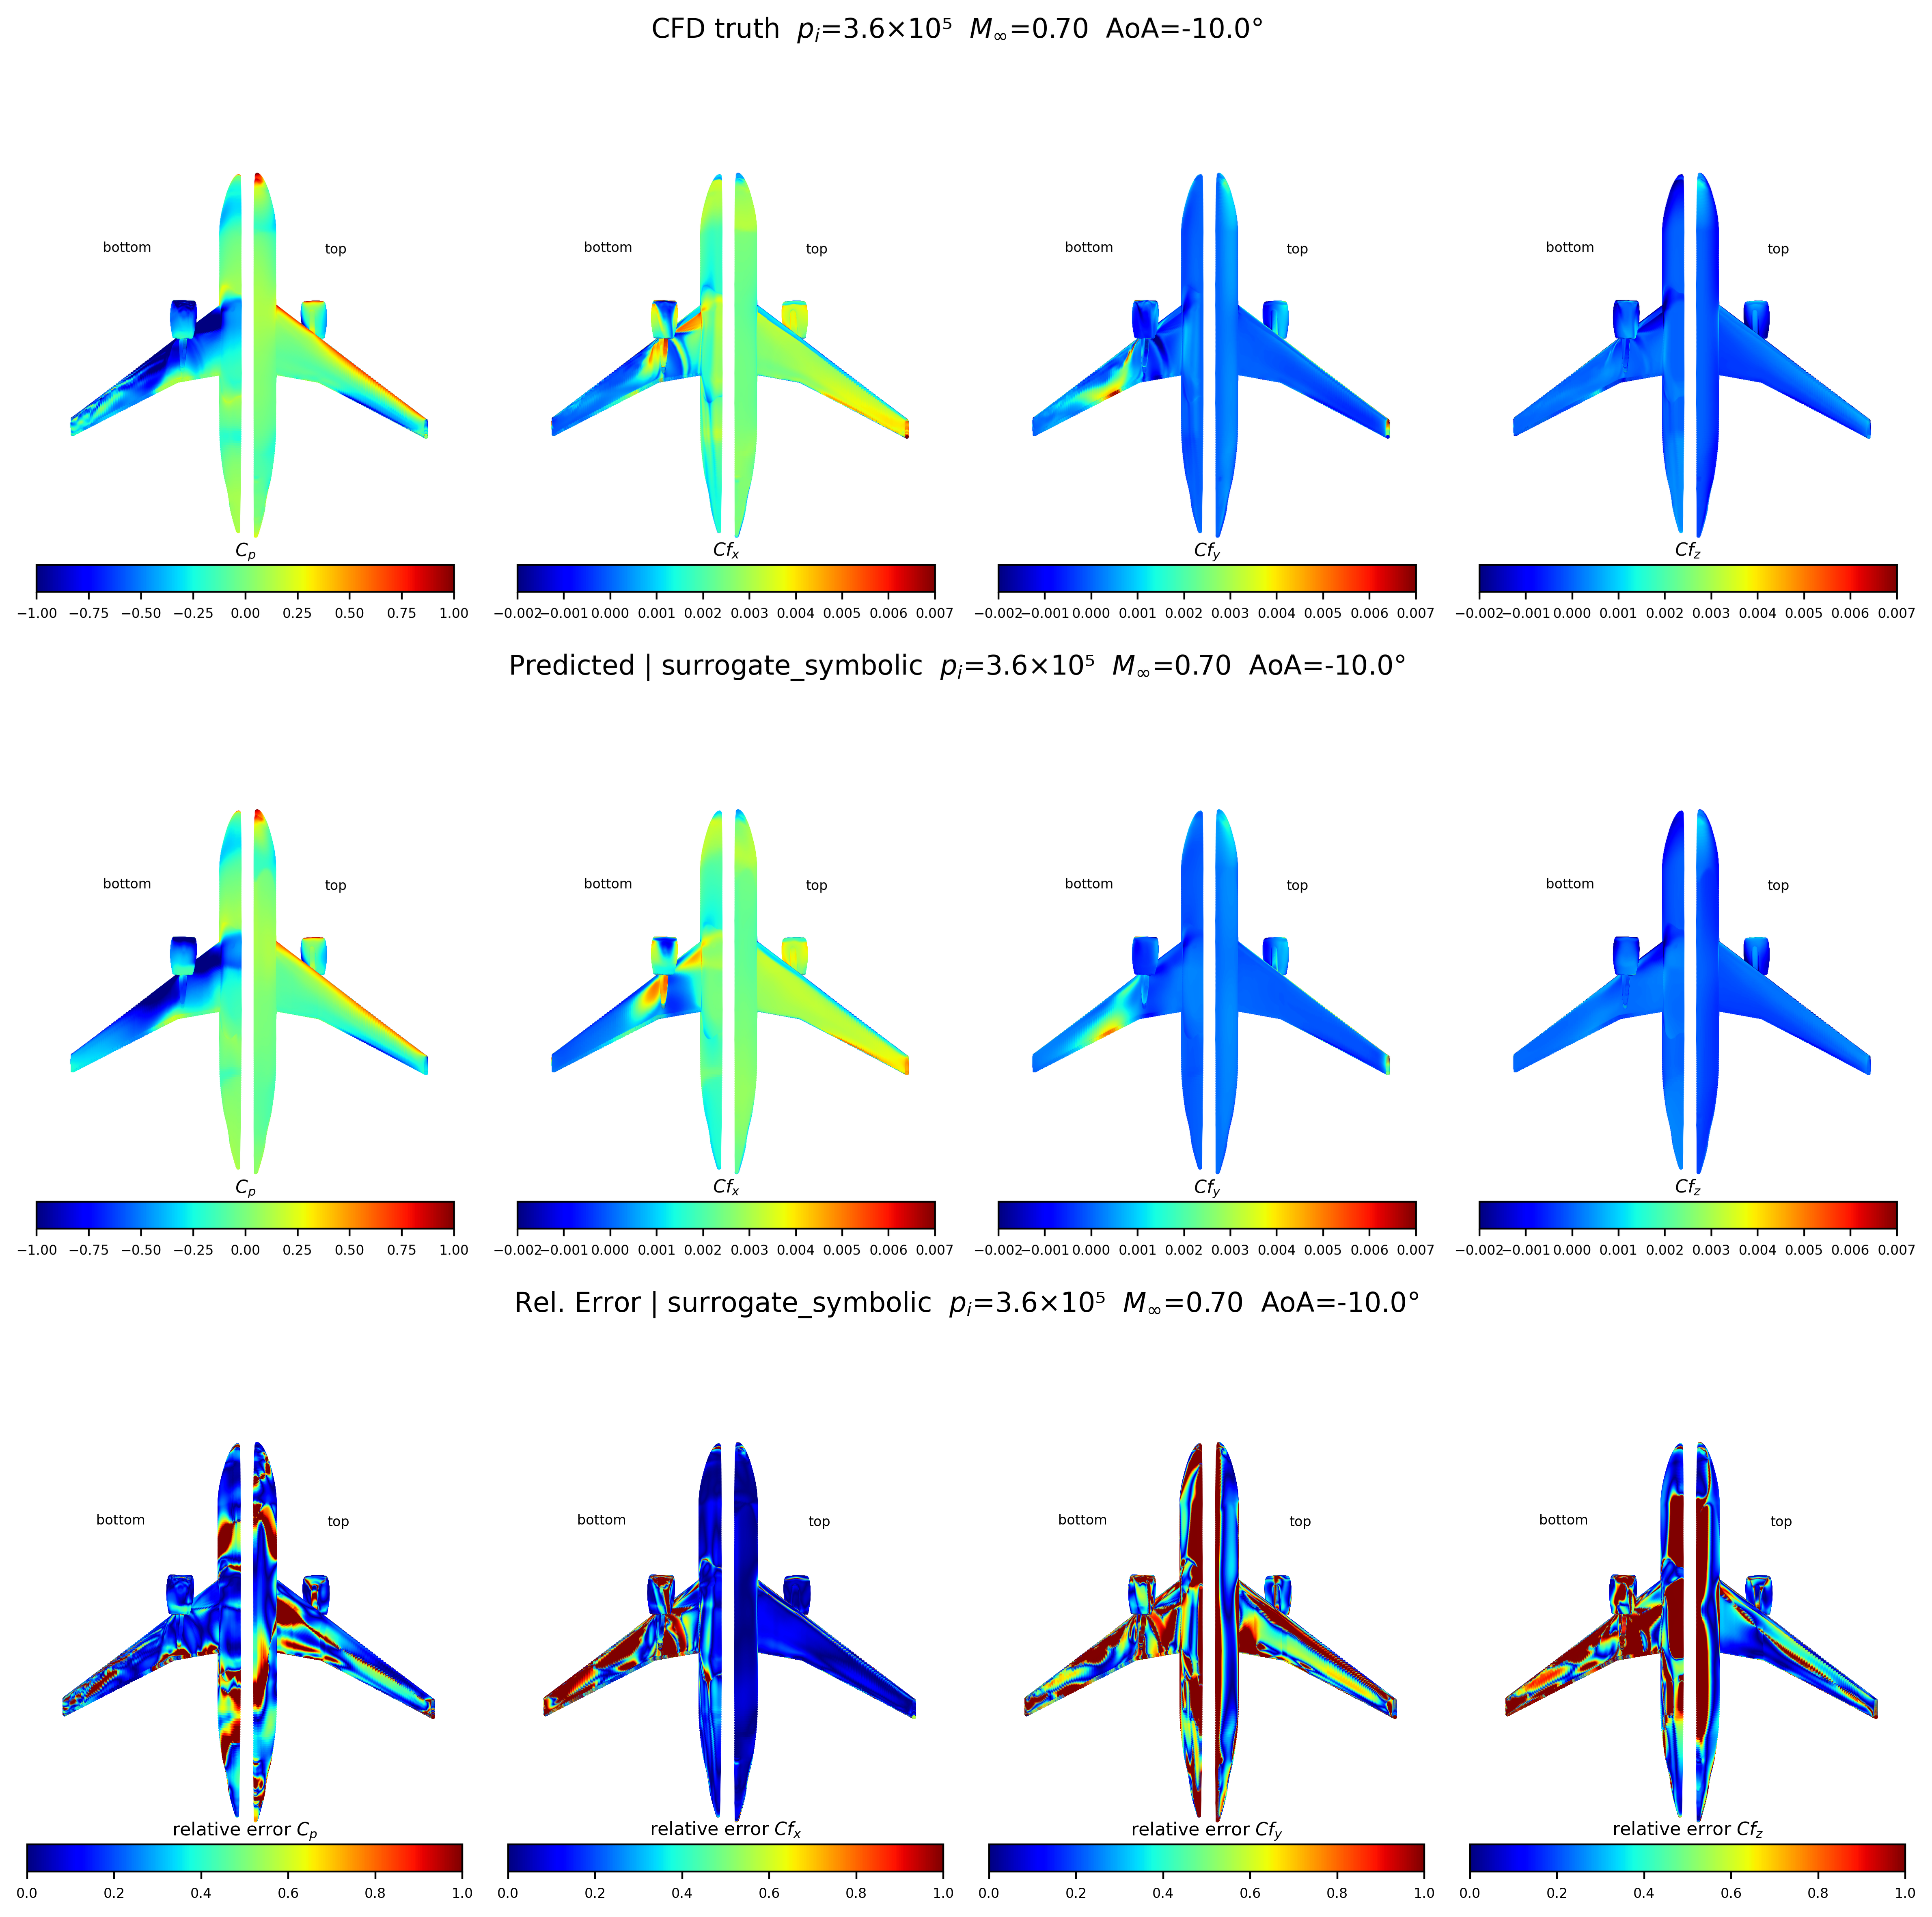
\includegraphics[width=0.88\textwidth]{figures/surface_fields_cond26.png}
\caption{High-subsonic, strong negative incidence ($M{=}0.70$,
  $\alpha{=}-10^{\circ}$, $\Pi{=}3.6{\times}10^{5}$): CFD reference
  (top), prediction (middle) and relative error (bottom).}
\label{fig:cond26}
\end{figure}

\begin{figure}[H]
\centering
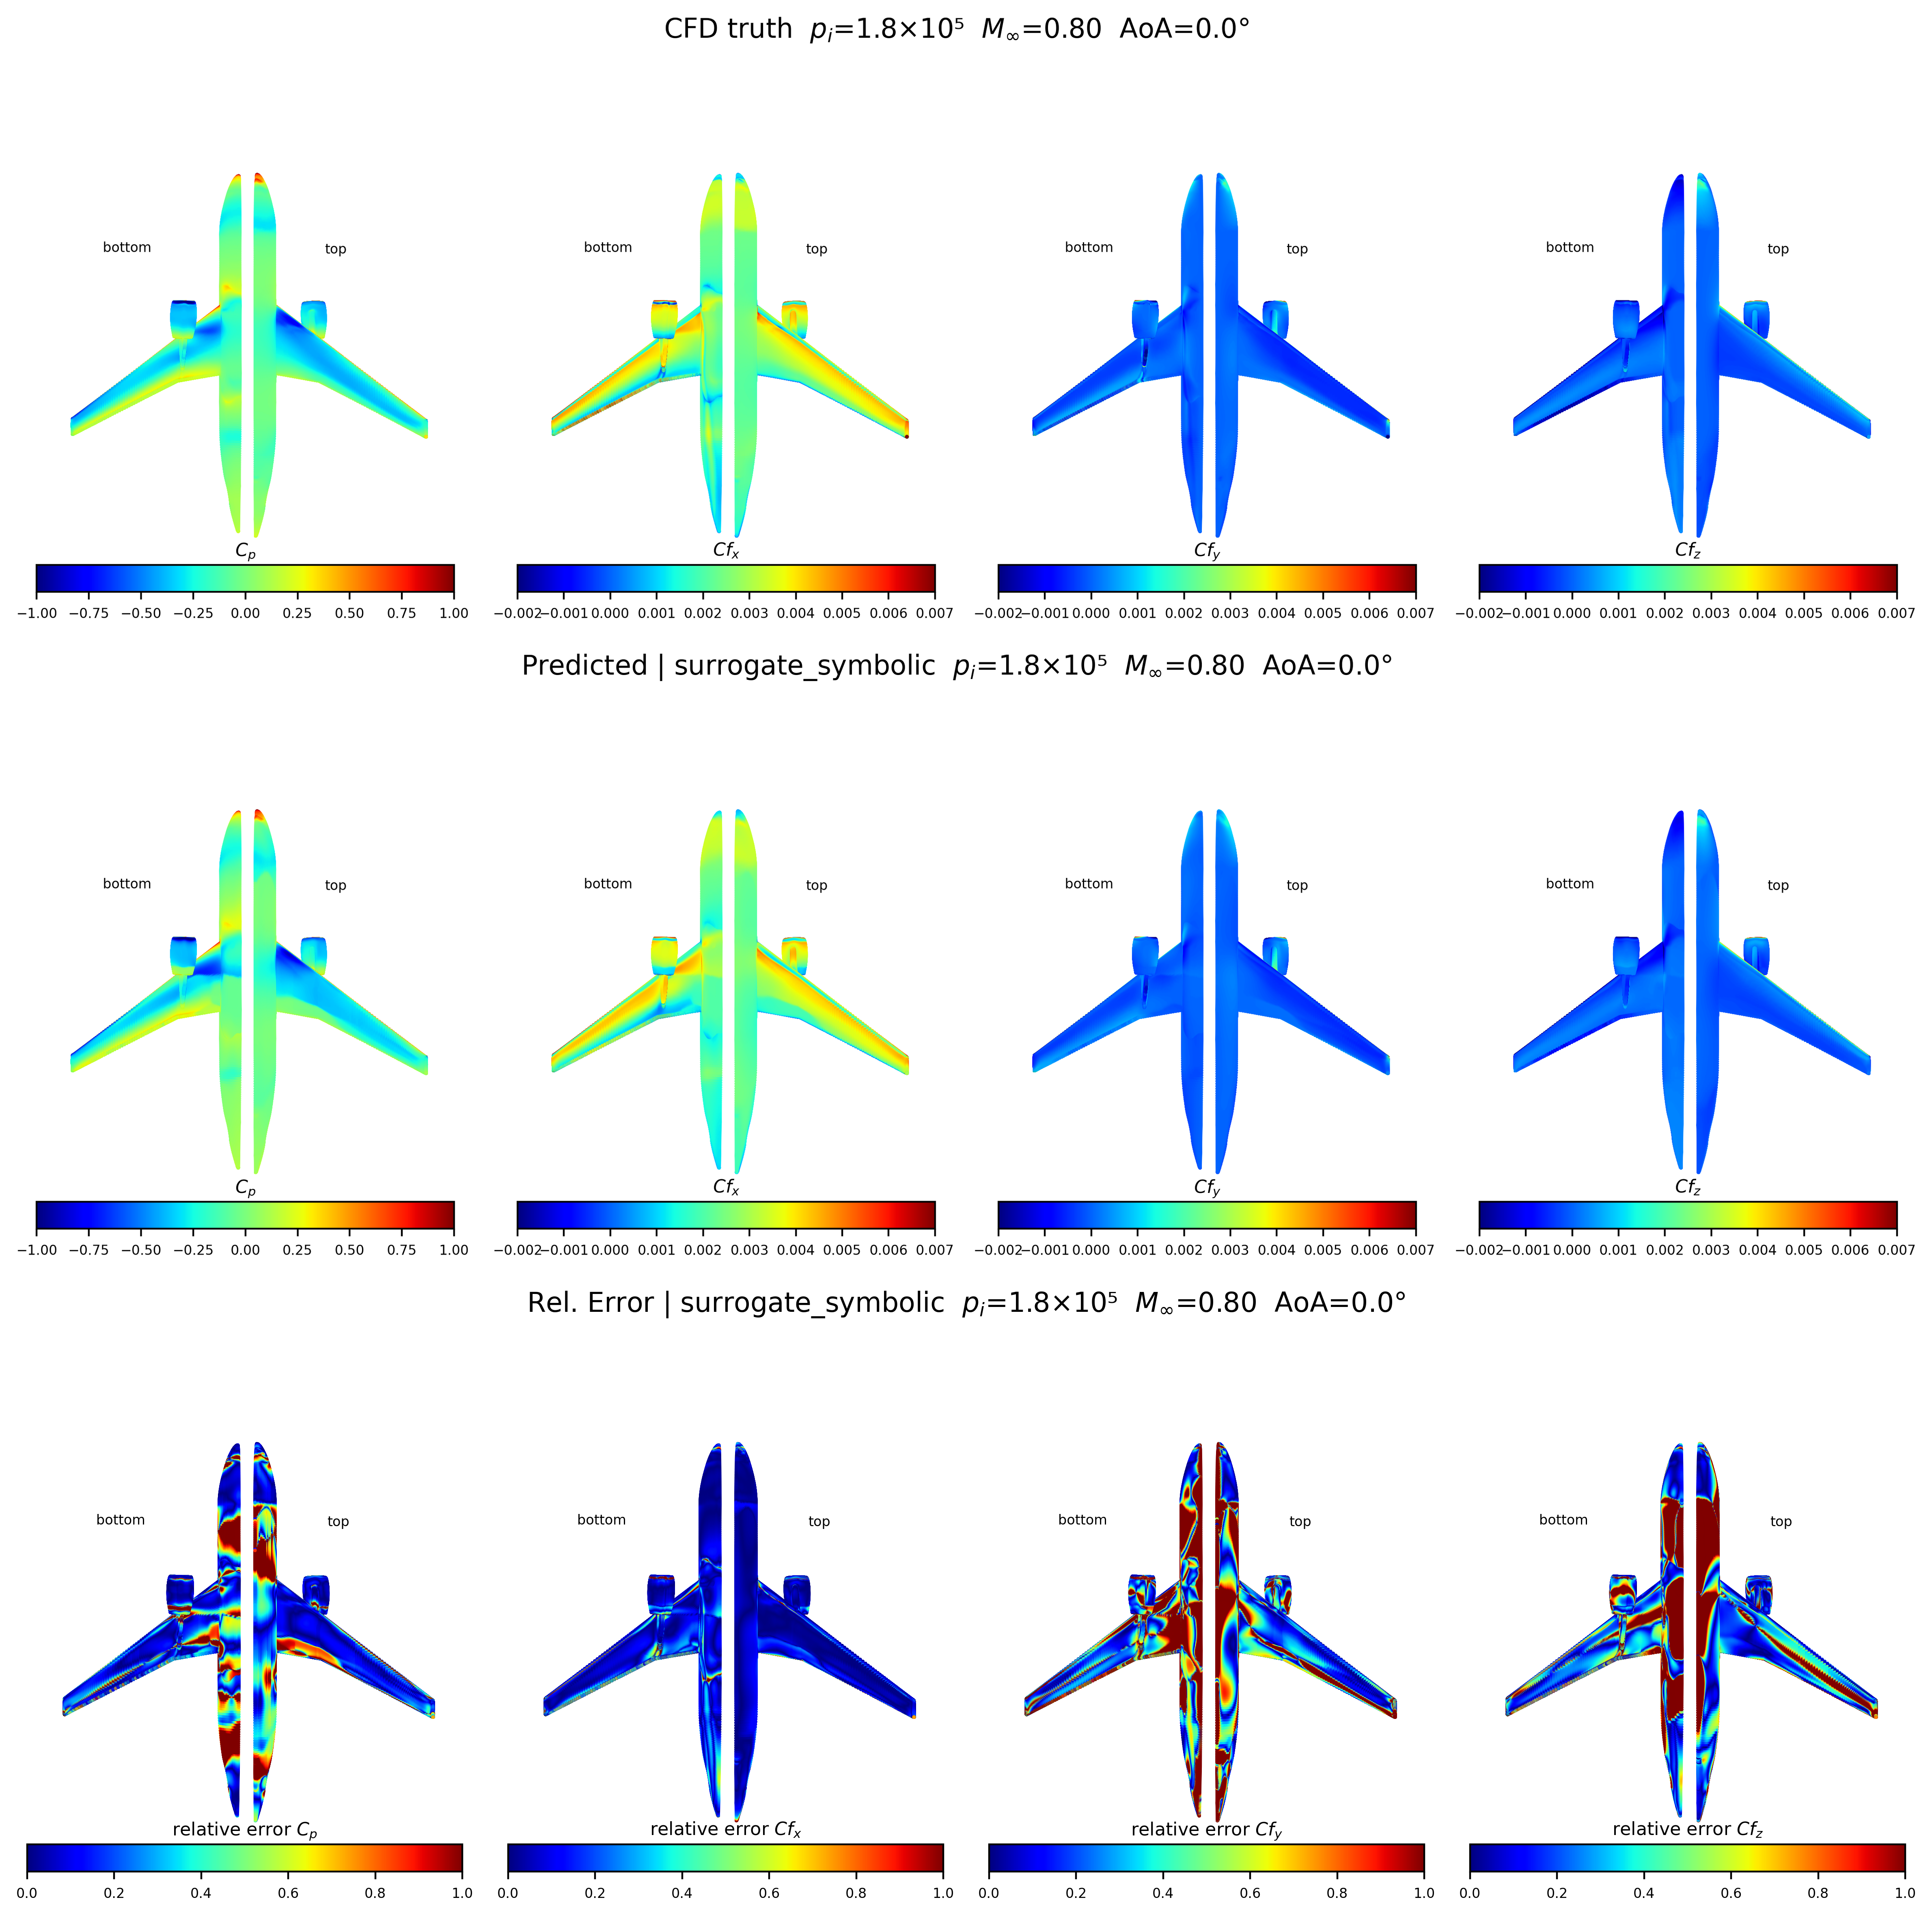
\includegraphics[width=0.88\textwidth]{figures/surface_fields_cond52.png}
\caption{Transonic cruise ($M{=}0.80$, $\alpha{=}0^{\circ}$,
  $\Pi{=}1.8{\times}10^{5}$): CFD reference (top), prediction
  (middle) and relative error (bottom).}
\label{fig:cond52}
\end{figure}

\begin{figure}[H]
\centering
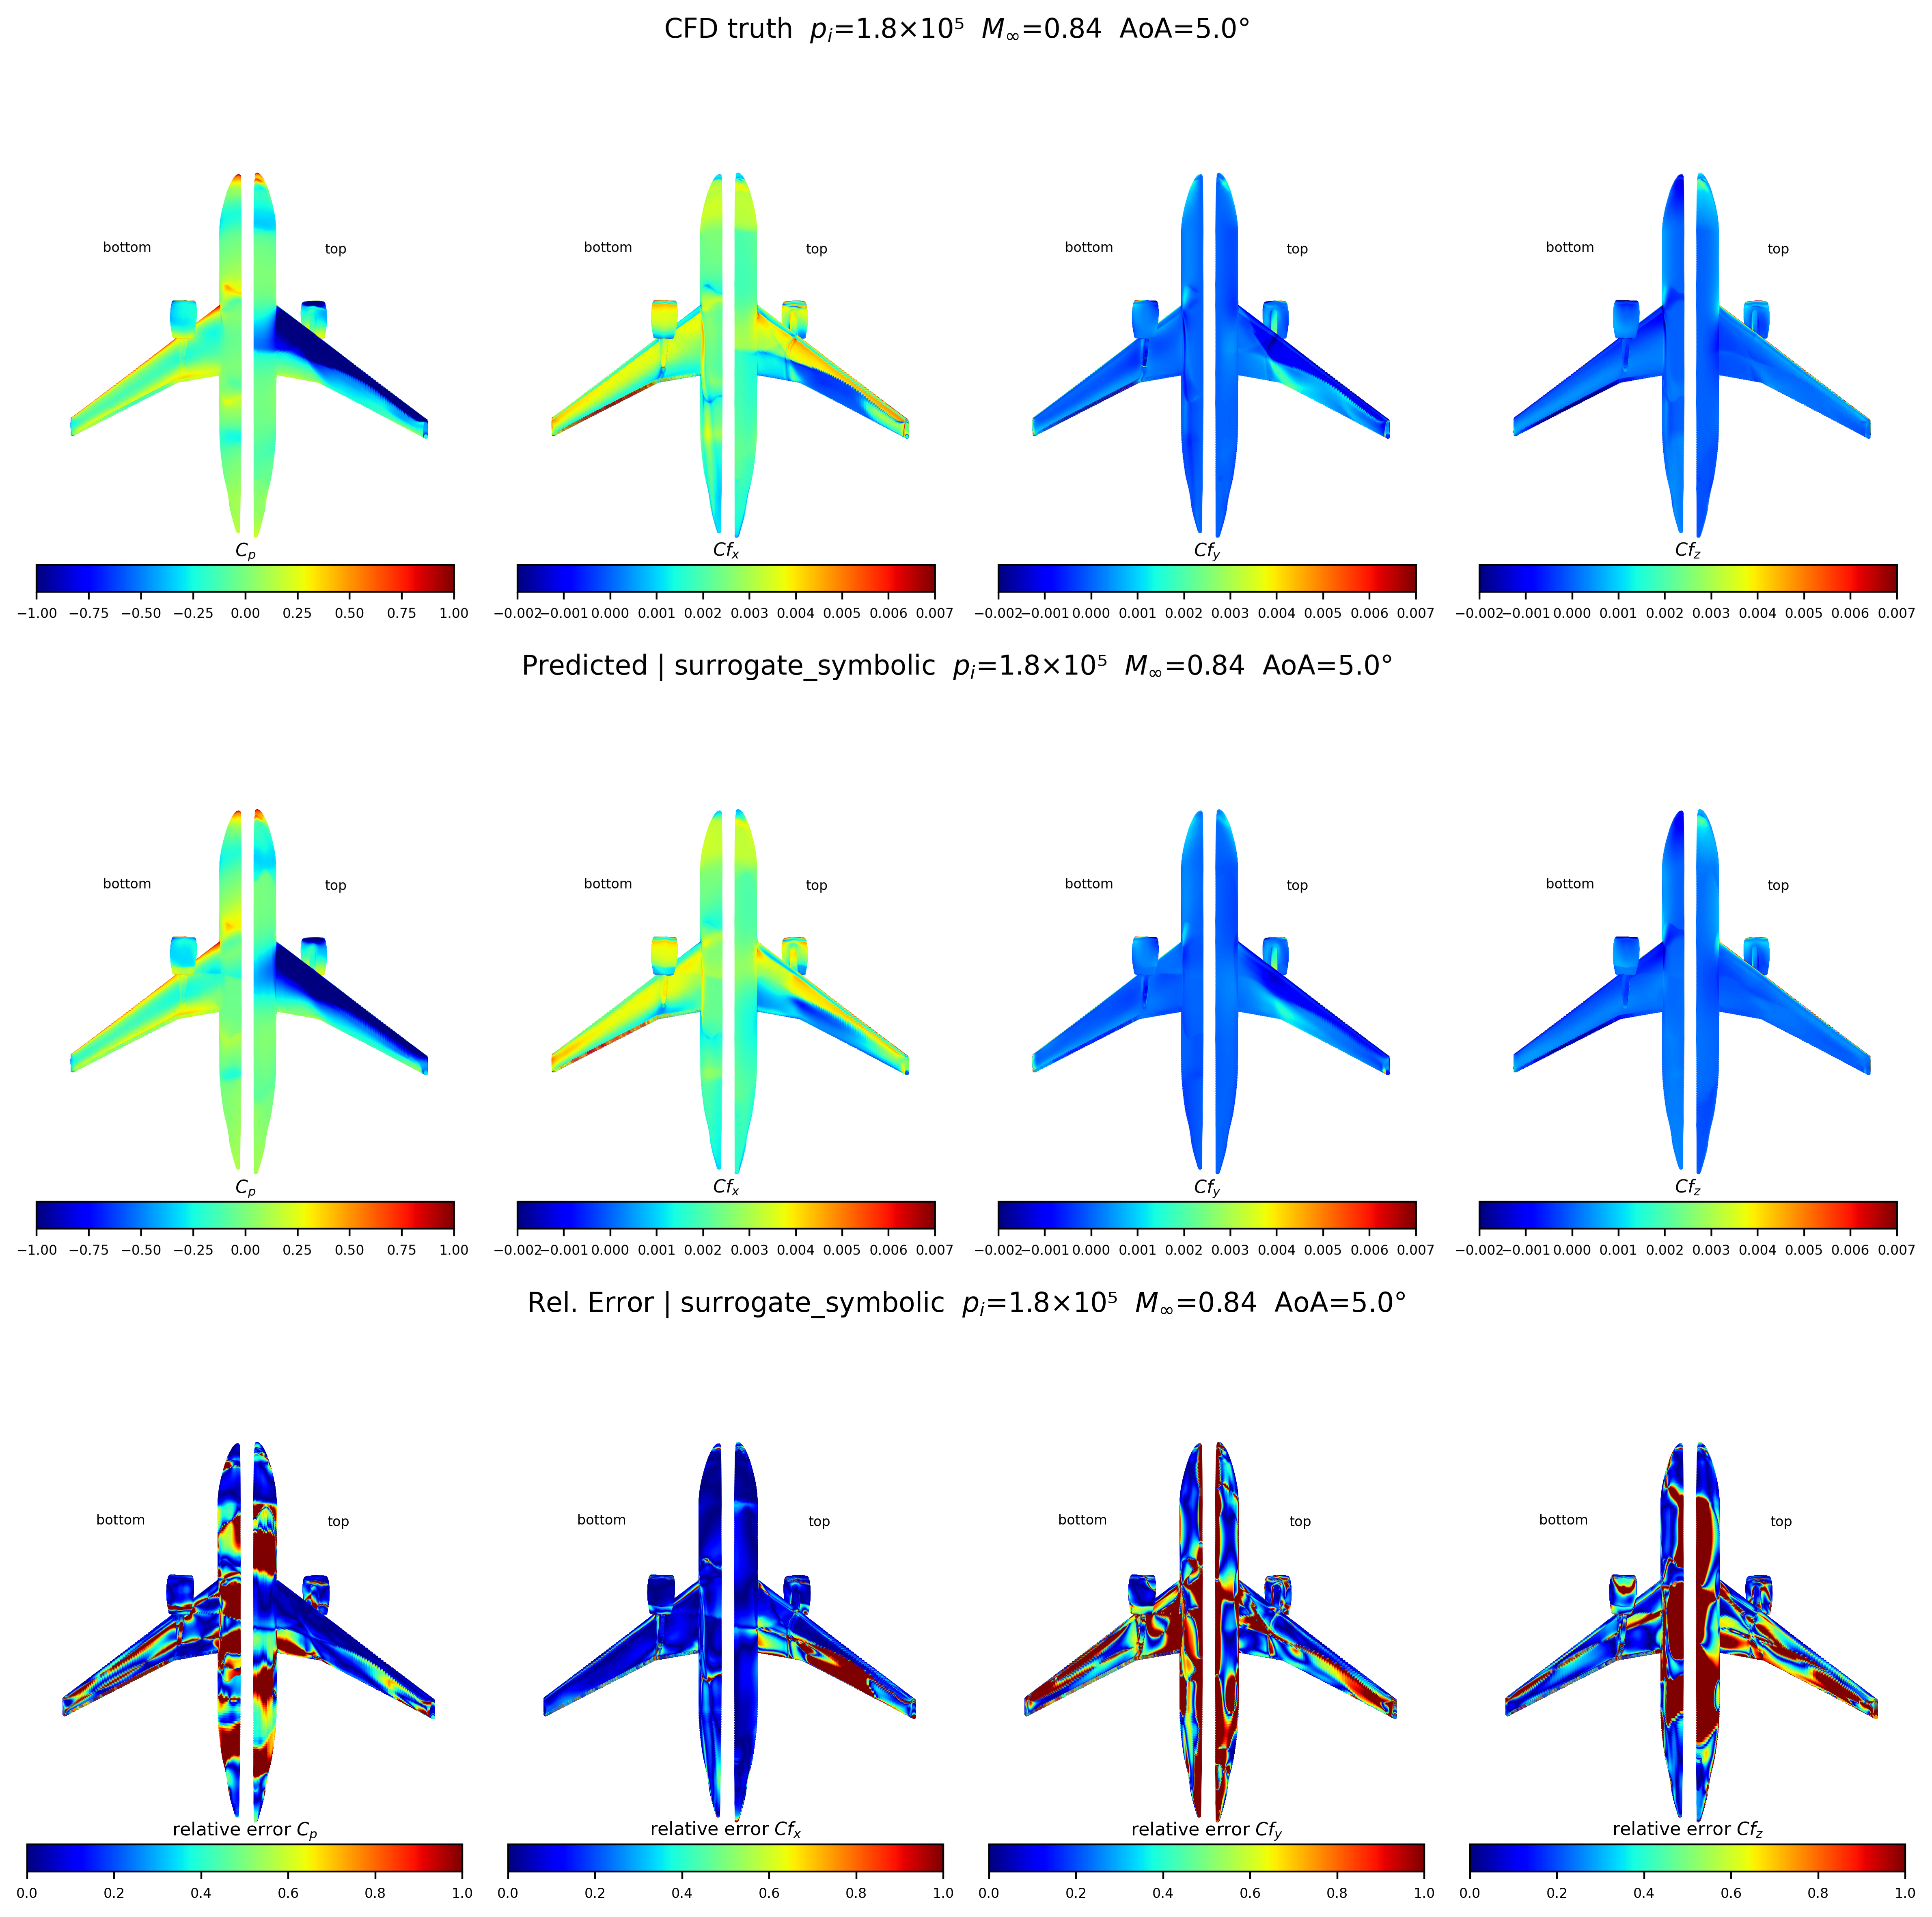
\includegraphics[width=0.88\textwidth]{figures/surface_fields_cond81.png}
\caption{Transonic, moderate incidence ($M{=}0.84$,
  $\alpha{=}5^{\circ}$, $\Pi{=}1.8{\times}10^{5}$): CFD reference
  (top), prediction (middle) and relative error (bottom).}
\label{fig:cond81}
\end{figure}

\begin{figure}[H]
\centering
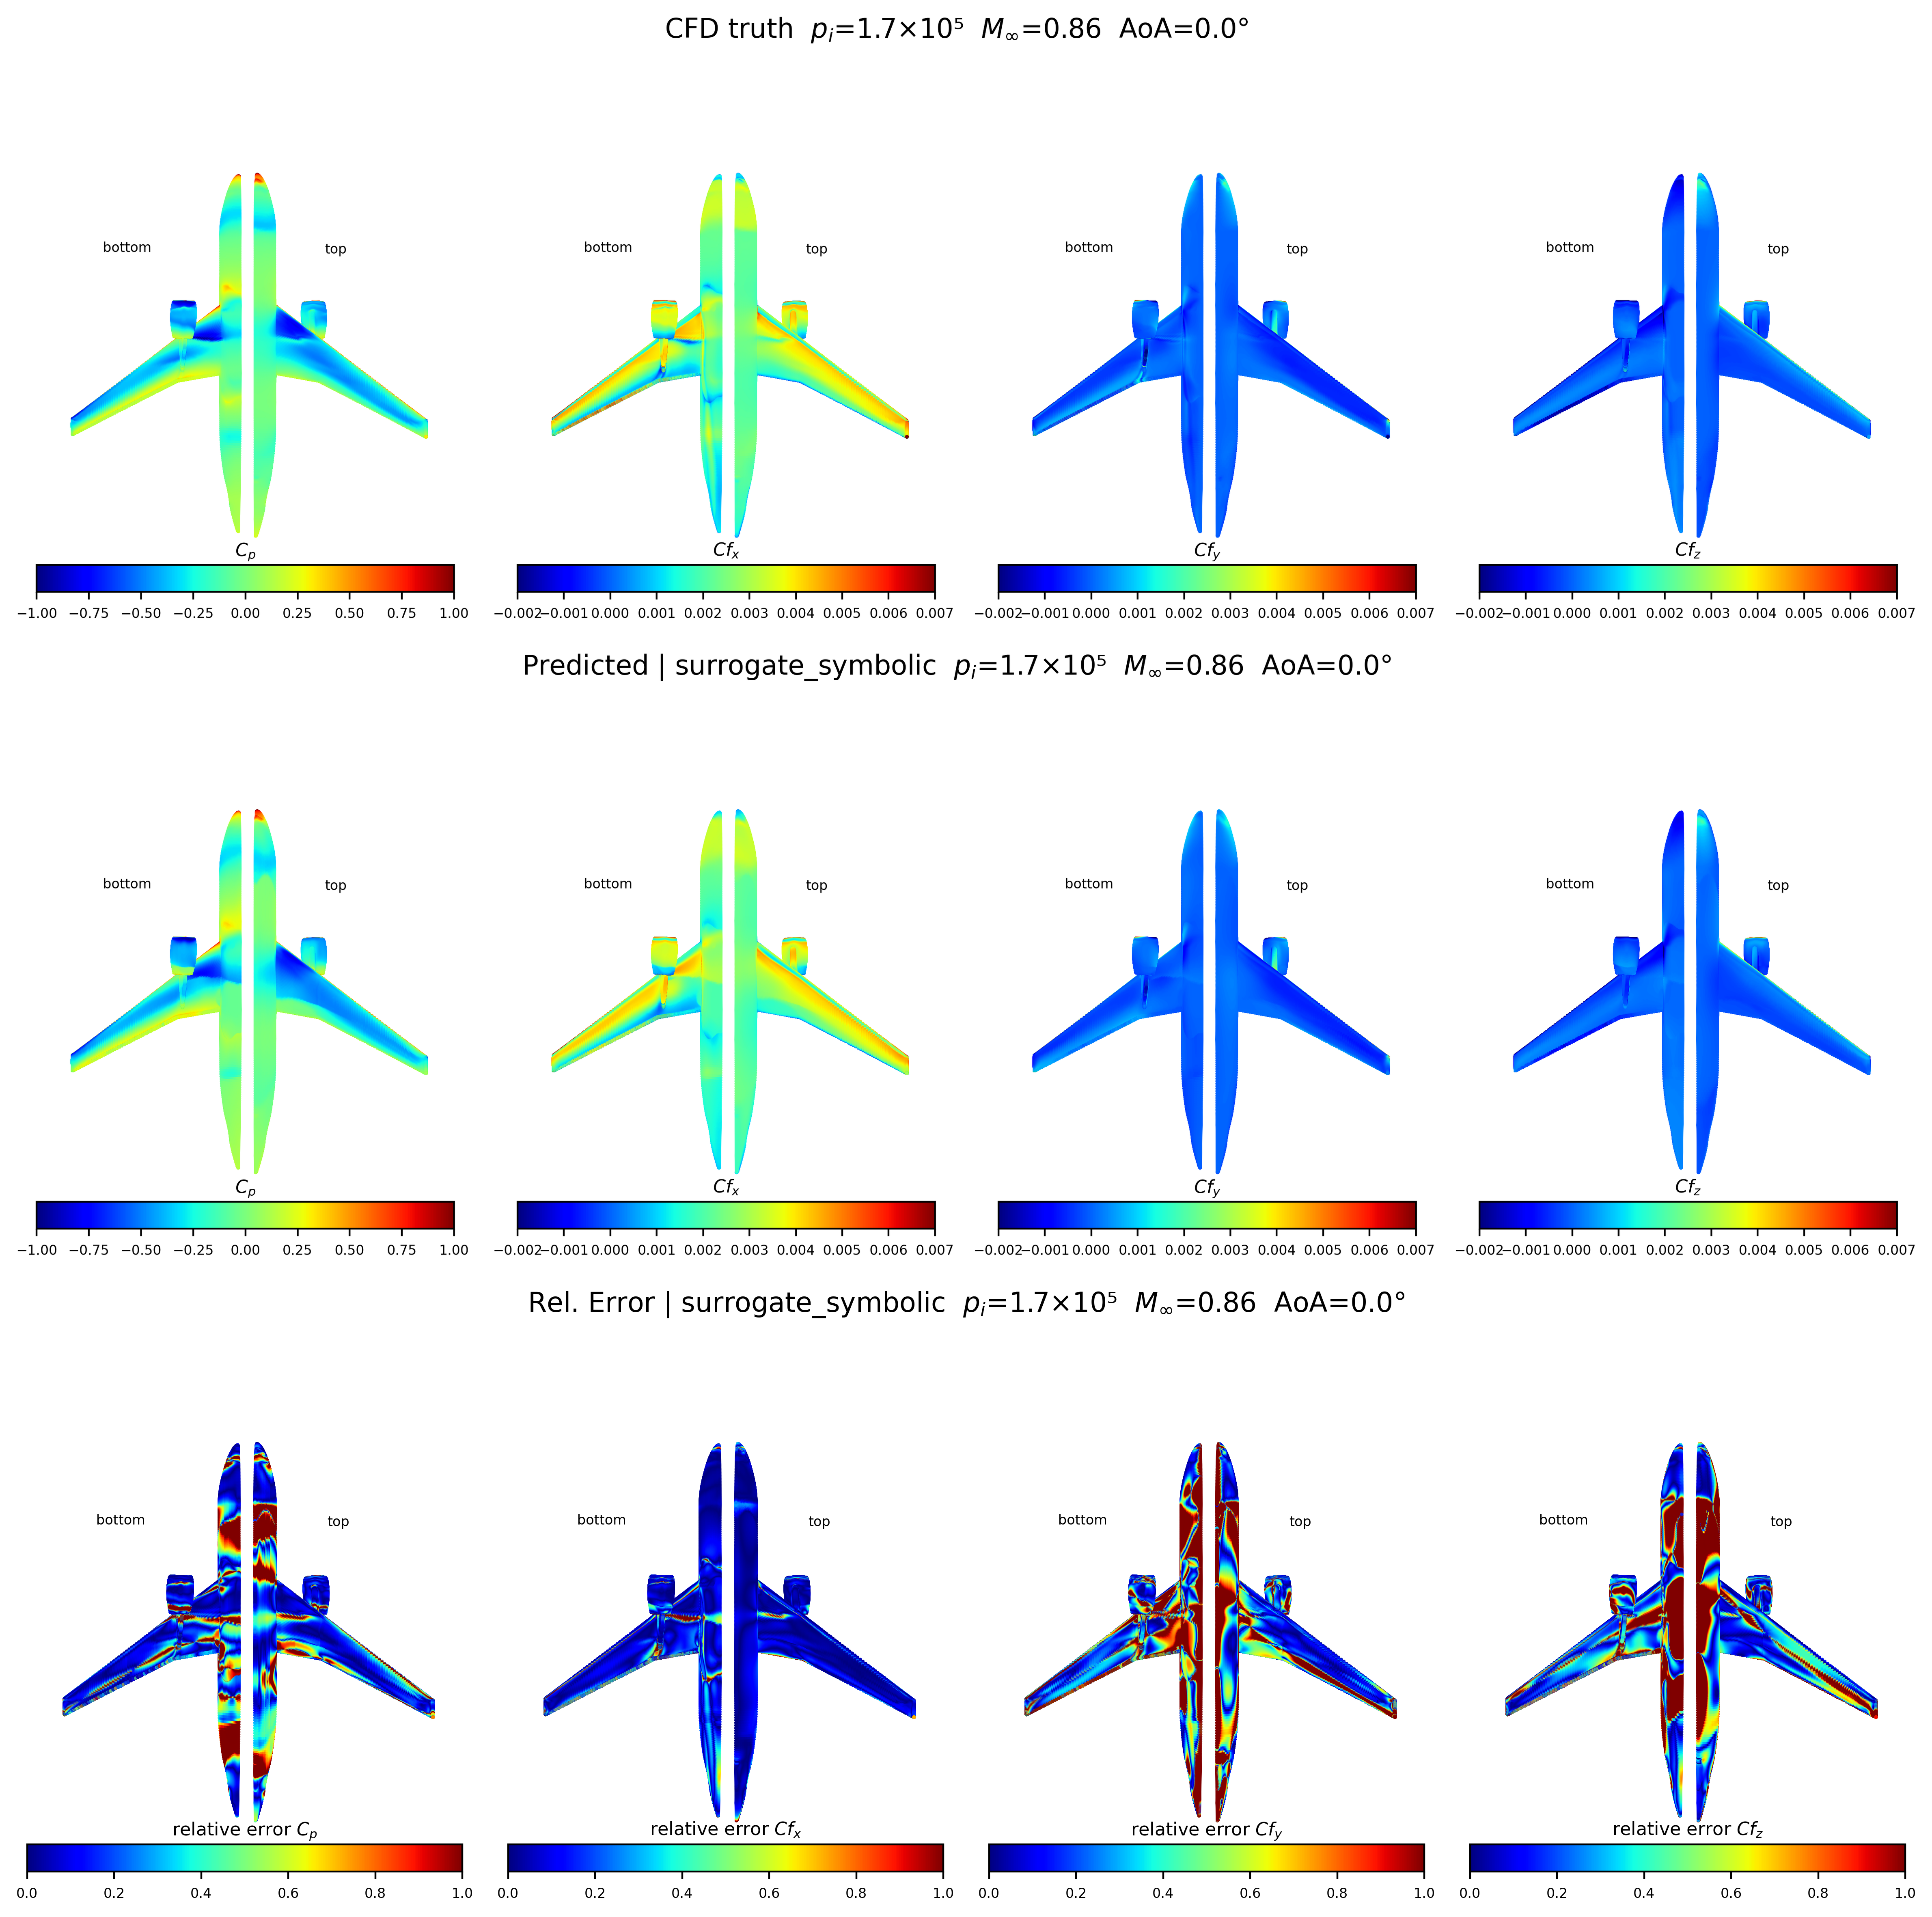
\includegraphics[width=0.88\textwidth]{figures/surface_fields_cond104.png}
\caption{High-transonic ($M{=}0.86$, $\alpha{=}0^{\circ}$,
  $\Pi{=}1.7{\times}10^{5}$): CFD reference (top), prediction
  (middle) and relative error (bottom).}
\label{fig:cond104}
\end{figure}

\begin{figure}[H]
\centering
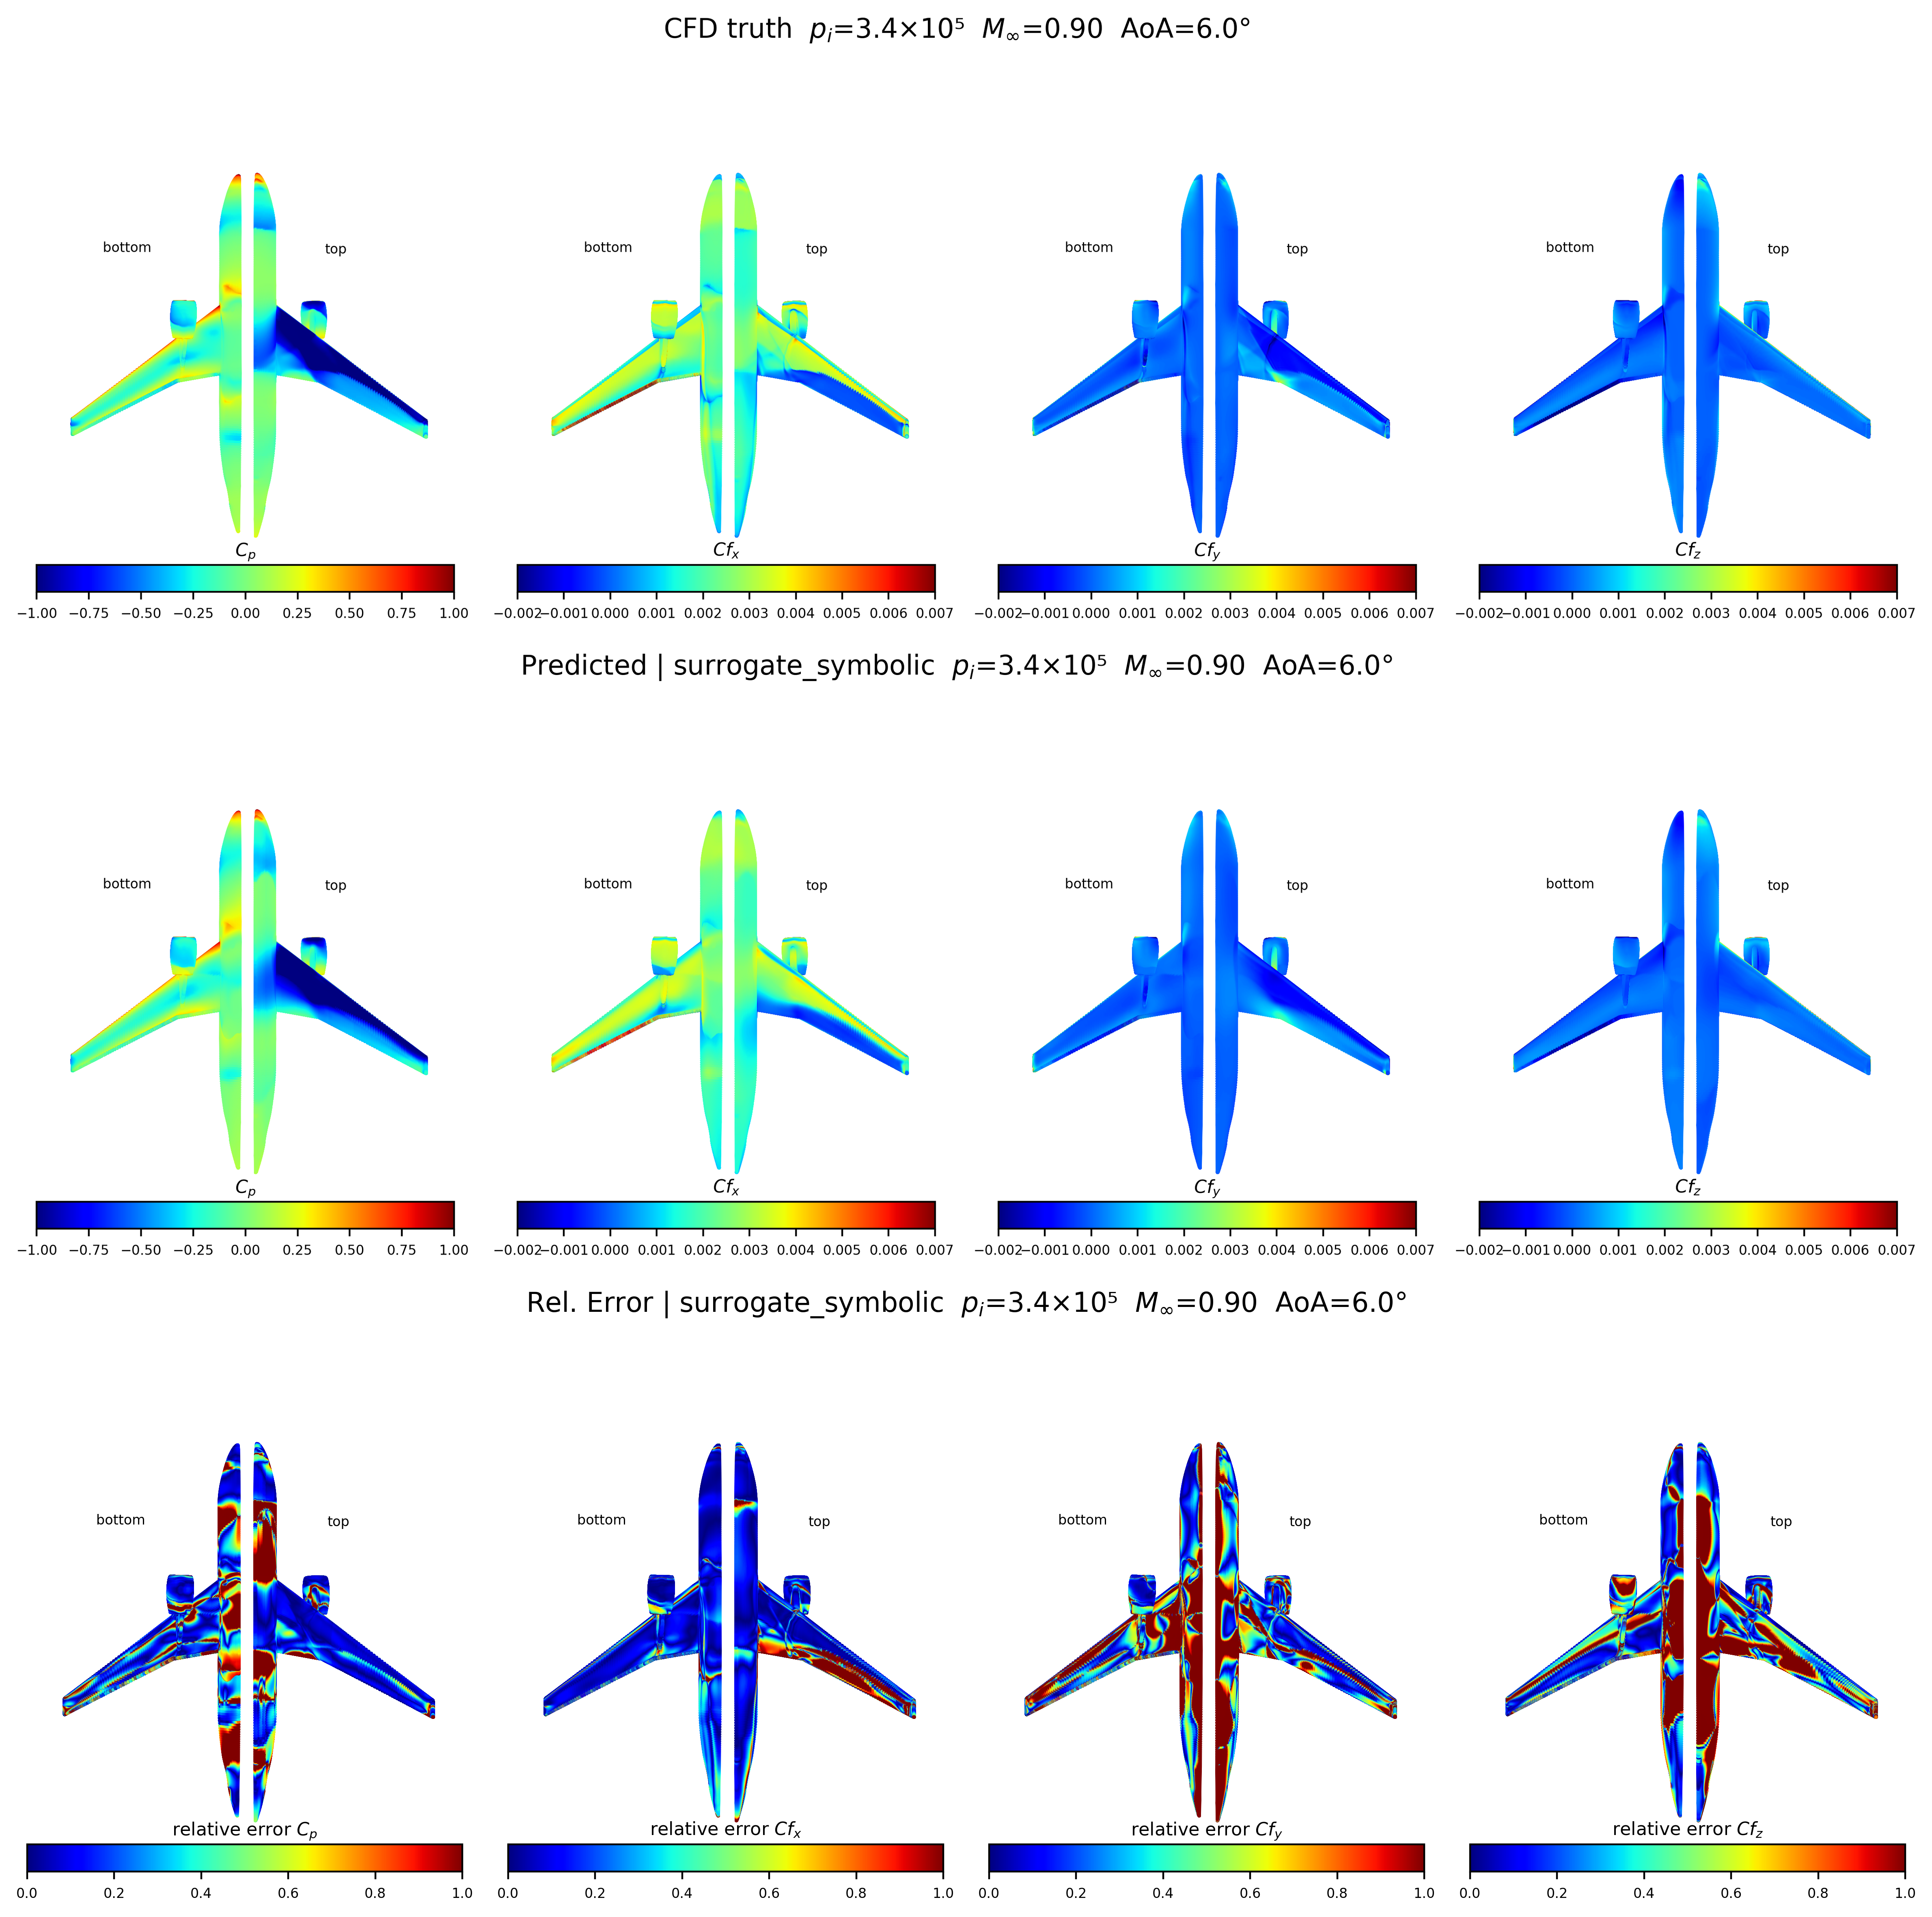
\includegraphics[width=0.88\textwidth]{figures/surface_fields_cond130.png}
\caption{High Mach, high incidence ($M{=}0.90$, $\alpha{=}6^{\circ}$,
  $\Pi{=}3.4{\times}10^{5}$): CFD reference (top), prediction
  (middle) and relative error (bottom).}
\label{fig:cond130}
\end{figure}

\subsection{Discussion}

Three aspects of the results merit emphasis.  First, the accuracy is
obtained \emph{pointwise} over a wide multi-regime envelope (Mach
0.30--0.96, AoA up to $\pm 15^{\circ}$) with a single compact model of
$3\times 10^{5}$ parameters, i.e.\ without per-condition retraining
or condition-specific calibration.  Second, the shock-weighted loss
and the shock-gated residual jointly address the smoothing pathology
at its source: during development, ablating either mechanism visibly
degraded the transonic $C_p$ reconstruction, with the plain-MLP
configuration smearing the pressure recovery across the shock.
Third, the symbolic gate demonstrates that interpretability need not
cost accuracy: the deployed model routes its experts with a five-node
formula whose variables---the critical pressure coefficient and the
span station---are exactly those an aerodynamicist would nominate,
and the formula was recovered from data rather than imposed.

% ================================================================
\section{CONCLUSIONS}
\label{sec:conclusions}
% ================================================================

A physics-aware, shock-gated Mixture of Experts surrogate for
transonic aerodynamic surface prediction has been presented and
evaluated on more than four million held-out RANS surface points of
the ONERA CRM WBPN configuration.  Four conclusions are drawn:

\begin{itemize}
  \item The shock-gated residual expert provides an explicit
        architectural mechanism for the pressure discontinuity,
        avoiding the shock-smoothing pathology of single smooth
        networks; combined with Mach-gated Gumbel-Softmax routing and
        a shock-weighted loss, the surrogate achieves
        $R^{2}(C_p)=0.9506$ and $R^{2}\approx 0.85$ on the three
        skin-friction components across Mach $0.30$--$0.96$ and
        AoA up to~$\pm 15^{\circ}$.
  \item Training labels derived from real RANS surface pressures via
        the critical-pressure criterion---rather than isentropic
        pseudo-labels computed from the inputs---give the shock
        probability a genuine physical meaning while keeping the
        inference path entirely solver-free.
  \item The LayerNorm + SiLU design eliminates the train/evaluation
        statistics gap observed with BatchNorm under heterogeneous
        flight-condition distributions, an implementation detail with
        first-order impact on deployed accuracy.
  \item Symbolic regression compresses the learned shock criterion
        into the closed-form expression
        $\tanh(\exp(C_p^{\mathrm{crit}}/\eta))$ (AUC-ROC 0.6727), and
        retraining with this frozen algebraic gate reproduces the
        neural-gate accuracy exactly---a data-driven confirmation
        that the network exploits genuine shock physics, and a route
        to fully interpretable, lightweight deployment.
\end{itemize}

Future work will extend the framework to multiple geometries to test
cross-geometry generalisation, incorporate unsteady RANS labels for
buffet-onset prediction, and exploit the differentiability of the
surrogate as a shock-aware penalty inside adjoint-based aerodynamic
shape optimisation loops.

% ================================================================
%  REFERENCES
% ================================================================

\begin{thebibliography}{26}

\bibitem{Vassberg2008}
J.C.~Vassberg, M.A.~DeHaan, S.M.~Rivers and R.A.~Wahls.
Development of a common research model for applied CFD validation
studies.
\textit{AIAA Paper 2008-6919}, 26th AIAA Applied Aerodynamics
Conference, Honolulu, HI, 2008.

\bibitem{Levy2013}
D.W.~Levy, K.R.~Laflin, E.N.~Tinoco, J.C.~Vassberg, M.~Mani,
B.~Rider, C.L.~Rumsey, R.A.~Wahls, J.H.~Morrison, O.P.~Brodersen,
S.~Crippa, D.J.~Mavriplis and M.~Murayama.
Summary of data from the fifth computational fluid dynamics drag
prediction workshop.
\textit{Journal of Aircraft}, Vol.~51, No.~4, pp.~1194--1213, 2014.

\bibitem{Peter2025}
J.~Peter, Q.~Bennehard, S.~Heib, J.-L.~Hantrais-Gervois and
F.~Mo\"ens.
ONERA's CRM WBPN database for machine learning activities, related
regression challenge and first results.
\textit{Computers \& Fluids}, 2025.  arXiv:2505.06265.

\bibitem{Han2018}
Z.-H.~Han, R.~Zhang and C.-Z.~Song.
Aerodynamic shape optimization of natural-laminar-flow wing using
surrogate-based approach.
\textit{Aerospace Science and Technology}, Vol.~74, pp.~51--60, 2018.

\bibitem{Bhatnagar2019}
S.~Bhatnagar, Y.~Afshar, S.~Pan, K.~Duraisamy and S.~Kaushik.
Prediction of aerodynamic flow fields using convolutional neural
networks.
\textit{Computational Mechanics}, Vol.~64, pp.~525--545, 2019.

\bibitem{Sekar2019}
V.~Sekar, Q.~Jiang, C.~Shu and B.C.~Khoo.
Fast flow field prediction over airfoils using deep learning approach.
\textit{Physics of Fluids}, Vol.~31, No.~5, 057103, 2019.

\bibitem{Ray2018}
D.~Ray and J.S.~Hesthaven.
An artificial neural network as a troubled-cell indicator.
\textit{Journal of Computational Physics}, Vol.~367, pp.~166--191, 2018.

\bibitem{Ray2019}
D.~Ray and J.S.~Hesthaven.
Detecting troubled-cells on two-dimensional unstructured grids using
a neural network.
\textit{Journal of Computational Physics}, Vol.~397, pp.~1--31, 2019.

\bibitem{Discacciati2020}
N.~Discacciati, J.S.~Hesthaven and D.~Ray.
Controlling oscillations in high-order discontinuous Galerkin schemes
using artificial viscosity tuned by neural networks.
\textit{Journal of Computational Physics}, Vol.~409, 109304, 2020.

\bibitem{Schwander2021}
L.~Schwander, D.~Ray and J.S.~Hesthaven.
Controlling oscillations in spectral methods by local artificial
viscosity governed by neural networks.
\textit{Journal of Computational Physics}, Vol.~431, 110144, 2021.

\bibitem{Morgan2020}
N.R.~Morgan, J.I.~Waltz, D.E.~Burton, M.R.J.~Charest,
T.R.~Canfield and J.G.~Wohlbier.
A Godunov-like point-centred essentially Lagrangian hydrodynamic
approach.
\textit{Journal of Computational Physics}, Vol.~408, 109298, 2020.

\bibitem{Raissi2019}
M.~Raissi, P.~Perdikaris and G.E.~Karniadakis.
Physics-informed neural networks: a deep learning framework for
solving forward and inverse problems involving nonlinear PDEs.
\textit{Journal of Computational Physics}, Vol.~378, pp.~686--707, 2019.

\bibitem{Karniadakis2021}
G.E.~Karniadakis, I.G.~Kevrekidis, L.~Lu, P.~Perdikaris, S.~Wang
and L.~Yang.
Physics-informed machine learning.
\textit{Nature Reviews Physics}, Vol.~3, pp.~422--440, 2021.

\bibitem{Brunton2016}
S.L.~Brunton, J.L.~Proctor and J.N.~Kutz.
Discovering governing equations from data by sparse identification
of nonlinear dynamical systems.
\textit{Proceedings of the National Academy of Sciences},
Vol.~113, No.~15, pp.~3932--3937, 2016.

\bibitem{Schmidt2009}
M.~Schmidt and H.~Lipson.
Distilling free-form natural laws from experimental data.
\textit{Science}, Vol.~324, No.~5923, pp.~81--85, 2009.

\bibitem{Cranmer2020}
M.~Cranmer, A.~Sanchez~Gonzalez, P.~Battaglia, R.~Xu, K.~Cranmer,
D.~Spergel and S.~Ho.
Discovering symbolic models from deep learning with inductive biases.
\textit{Advances in Neural Information Processing Systems},
Vol.~33, 2020.

\bibitem{LaCava2021}
W.~La~Cava, P.~Orzechowski, B.~Burlacu, F.O.~de~Franca,
M.~Virgolin, Y.~Jin, M.~Kommenda and J.H.~Moore.
Contemporary symbolic regression methods and their relative
performance.
\textit{Advances in Neural Information Processing Systems},
Vol.~34, 2021.

\bibitem{Angelis2023}
D.~Angelis, F.~Sofos and T.E.~Karakasidis.
Artificial intelligence in physical sciences: symbolic regression
trends and perspectives.
\textit{Archives of Computational Methods in Engineering},
Vol.~30, pp.~3845--3865, 2023.

\bibitem{Jacobs1991}
R.A.~Jacobs, M.I.~Jordan, S.J.~Nowlan and G.E.~Hinton.
Adaptive mixtures of local experts.
\textit{Neural Computation}, Vol.~3, No.~1, pp.~79--87, 1991.

\bibitem{Shazeer2017}
N.~Shazeer, A.~Mirhoseini, K.~Maziarz, A.~Davis, Q.~Le,
G.~Hinton and J.~Dean.
Outrageously large neural networks: the sparsely-gated
mixture-of-experts layer.
\textit{International Conference on Learning Representations}, 2017.

\bibitem{Fedus2022}
W.~Fedus, B.~Zoph and N.~Shazeer.
Switch Transformers: scaling to trillion parameter models with
simple and efficient sparsity.
\textit{Journal of Machine Learning Research}, Vol.~23, No.~120,
pp.~1--39, 2022.

\bibitem{Jang2017}
E.~Jang, S.~Gu and B.~Poole.
Categorical reparameterization with Gumbel-Softmax.
\textit{International Conference on Learning Representations}, 2017.

\bibitem{Maddison2017}
C.J.~Maddison, A.~Mnih and Y.W.~Teh.
The Concrete distribution: a continuous relaxation of discrete
random variables.
\textit{International Conference on Learning Representations}, 2017.

\bibitem{Ba2016}
J.L.~Ba, J.R.~Kiros and G.E.~Hinton.
Layer normalization.
\textit{arXiv preprint arXiv:1607.06450}, 2016.

\bibitem{Elfwing2018}
S.~Elfwing, E.~Uchibe and K.~Doya.
Sigmoid-weighted linear units for neural network function
approximation in reinforcement learning.
\textit{Neural Networks}, Vol.~107, pp.~3--11, 2018.

\bibitem{Ramachandran2017}
P.~Ramachandran, B.~Zoph and Q.V.~Le.
Searching for activation functions.
\textit{arXiv preprint arXiv:1710.05941}, 2017.

\end{thebibliography}

\end{document}
